% !TeX TXS-program:bibliography = txs:///biber
\documentclass[14pt, russian]{scrartcl}
\let\counterwithout\relax
\let\counterwithin\relax

\usepackage{float}
\usepackage{xcolor}
\usepackage{extsizes}
\usepackage{subfig}
\usepackage[export]{adjustbox}
\usepackage{tocvsec2} % глубина разделов в оглавлении
\usepackage[subfigure]{tocloft} % сетка из картинок
\usepackage[newfloat]{minted} % можно менять место, где располагать объект
\captionsetup[listing]{position=top} % настрокйка подписи 

% команды ниже просто добавляют перед текстам нечто
\AtBeginEnvironment{figure}{\vspace{0.5cm}}
\AtBeginEnvironment{table}{\vspace{0.5cm}}
\AtBeginEnvironment{listing}{\vspace{0.5cm}}
\AtBeginEnvironment{algorithm}{\vspace{0.5cm}}
\AtBeginEnvironment{minted}{\vspace{-0.5cm}}

\usepackage{fancyvrb}
\usepackage{ulem,bm,mathrsfs,ifsym} %зачеркивания, особо жирный стиль и RSFS начертание
\usepackage{sectsty} % переопределение стилей подразделов

% для полей и разметки страницы
\usepackage{pdflscape} %альбомные страницы
\usepackage{geometry} % настройка размеров страниц              
\geometry{a4paper, tmargin=2cm, bmargin=2cm, lmargin=3cm, rmargin=1cm} % тоже самое, но лучше

% математика
\usepackage{amsthm,amsfonts,amsmath,amssymb,amscd}  % дополнения от AMS
\usepackage{mathtools} % добавляет окружение multlined
\usepackage[perpage]{footmisc} % нумперация сносок на каждой странице 
\KOMAoptions{fontsize=14pt} % изменение параметров страницы 

\makeatletter % для команды с символом @ в имени не в стилевом пакете, а прямо в тексте документа
\def\showfontsize{\f@size{} point}
\makeatother

% про стили и языки 
\usepackage{tempora} % шрифт times
\usepackage{cmap} % улучшает поиск кирилицы в pdf
\usepackage[T1]{fontenc} % поддержка русских букв
\usepackage[utf8]{inputenc} % кодировка utf8
\usepackage[english, main=russian]{babel} % языки: русский, английский

% оформление текста
\usepackage{indentfirst} % красная строка

% таблицы
\usepackage{longtable} % длинные таблицы
\usepackage{multirow, makecell, array} % улучшенное форматирование таблиц
\usepackage{booktabs} % возможность оформления таблиц в классическом книжном стиле (при правильном использовании не противоречит ГОСТ)

% общее форматирование
\usepackage{soulutf8} % переносоустойчивые подчёркивания и зачёркивания
\usepackage{icomma} % запятая в десятичных дробях

% картинки
\usepackage{graphicx} % работа с графикой
\usepackage{wrapfig} % картинки могут «обтекаться» текстом 

% списки
\usepackage{enumitem}

% подписи 
\usepackage{caption} % помогает настраивать подписи к рисункам и таблицам                       
%% Использование:
%\begin{table}[h!]\ContinuedFloat - чтобы не переключать счетчик
%\captionsetup{labelformat=continued} %должен стоять до самого caption
%\caption{}
% либо ручками \caption*{Продолжение таблицы~\ref{...}.} :)

% интервалы
\addto\captionsrussian{
  \renewcommand{\listingname}{Листинг}
}

%счётчики
\usepackage[figure, table, section]{totalcount} % счётчик рисунков и таблиц
\DeclareTotalCounter{lstlisting} % считать листинги тоже
\usepackage{totcount} % создание счётчиков на основе последнего номера подсчитываемого элемента 
\usepackage{totpages} % счётчик страниц, совместимый с hyperref (ссылается на номер последней страницы) 

% интервалы
% linespread-реализация ближе к реализации полуторного интервала в ворде.
% setspace реализация заточена под шрифты 10, 11, 12pt, под остальные кегли хуже, но всё же ближе к типографской классике. 
\linespread{1.3} % Полуторный интервал (ГОСТ Р 7.0.11-2011, 5.3.6)
%\renewcommand{\@biblabel}[1]{#1}

% гиперссылки
\usepackage{hyperref}

% выравнивание и переносы
\sloppy % оберег от переполнений 
\clubpenalty=10000 % запрет разрыва страницы после первой строки абзаца
\widowpenalty=10000 % запрет разрыва страницы после последней строки абзаца

% какая-то магия
\makeatletter % малые заглавные, small caps shape
\let\@@scshape=\scshape
\renewcommand{\scshape}{%
  \ifnum\strcmp{\f@series}{bx}=\z@
    \usefont{T1}{cmr}{bx}{sc}%
  \else
    \ifnum\strcmp{\f@shape}{it}=\z@
      \fontshape{scsl}\selectfont
    \else
      \@@scshape
    \fi
  \fi}
\makeatother

% подписи 
%\captionsetup{%
%singlelinecheck=off, % многострочные подписи, например у таблиц
%skip=2pt, % вертикальная отбивка между подписью и содержимым рисунка или таблицы определяется ключом
%justification=centering, % центрирование подписей, заданных командой \caption
%}

% пакеты
\usepackage{ifthen} % добавляет ifthenelse
% инициализирование переменных, не трогать! (опять магия)
\newcounter{intvl}
\newcounter{otstup}
\newcounter{contnumeq}
\newcounter{contnumfig}
\newcounter{contnumtab}
\newcounter{pgnum}
\newcounter{bibliosel}
\newcounter{chapstyle}
\newcounter{headingdelim}
\newcounter{headingalign}
\newcounter{headingsize}
\newcounter{tabcap}
\newcounter{tablaba}
\newcounter{tabtita}
%%%%%%%%%%%%%%%%%%%%%%%%%%%%%%%%%%%%%%%%%%%%%%%%%%
%%% Область упрощённого управления оформлением %%%

% интервал между заголовками и между заголовком и текстом
% заголовки отделяют от текста сверху и снизу тремя интервалами (ГОСТ Р 7.0.11-2011, 5.3.5)
\setcounter{intvl}{3} % коэффициент кратности к размеру шрифта

% отступы у заголовков в тексте
\setcounter{otstup}{0} % 0 - без отступа; 1 - абзацный отступ

% нумерация формул, таблиц и рисунков
\setcounter{contnumeq}{1} % нумерация формул: 0 - пораздельно, 1 - сквозная нумерация по всему документу
\setcounter{contnumfig}{1} % нумерация рисунков: 0 - пораздельно, 1 - сквозная нумерация по всему документу
\setcounter{contnumtab}{1} % нумерация таблиц: 0 - пораздельно, 1 - сквозная нумерация по всему документу

% оглавление
\setcounter{pgnum}{0} % 0 - номера страниц никак не обозначены, 1 - стр. над номерами страниц

% библиография
\setcounter{bibliosel}{1} % 0 - встроенная реализация с загрузкой файла через движок bibtex8, 1 - реализация пакетом biblatex через движок biber

% текст и форматирование заголовков
\setcounter{chapstyle}{1} % 0 - разделы только под номером, 1 - разделы с названием "Глава" перед номером
\setcounter{headingdelim}{1} % 0 - номер отделен пропуском в 1em или \quad, 1 - номера разделов и приложений отделены точкой с пробелом, подразделы пропуском без точки, 2 - номера разделов, подразделов и приложений отделены точкой с пробелом

% выравнивание заголовков в тексте
\setcounter{headingalign}{0} % 0 - по центру, 1 - по левому краю

% размеры заголовков в тексте
\setcounter{headingsize}{0} % 0 - по ГОСТ, все всегда 14 пт; 1 - пропорционально изменяющийся размер в зависимости от базового шрифта

% подпись таблиц
\setcounter{tabcap}{0} % 0 - по ГОСТ, номер таблицы и название разделены тире, выровнены по левому краю, при необходимости на нескольких строках, 1 - подпись таблицы не по ГОСТ, на двух и более строках, дальнейшие настройки: 
% выравнивание первой строки, с подписью и номером
\setcounter{tablaba}{2} % 0 - по левому краю, 1 - по центру, 2 - по правому краю
% выравнивание строк с самим названием таблицы
\setcounter{tabtita}{1} % 0 - по левому краю, 1 - по центру, 2 - по правому краю

% картинки
\DeclareCaptionLabelSeparator*{emdash}{~--- } % (ГОСТ 2.105, 4.3.1)
\captionsetup[figure]{labelsep=emdash,font=onehalfspacing,position=bottom}

% таблицы
\ifthenelse{\equal{\thetabcap}{0}}{
    \newcommand{\tabcapalign}{\raggedright} % по левому краю страницы или аналога parbox
}

\ifthenelse{\equal{\thetablaba}{0} \AND \equal{\thetabcap}{1}}{
    \newcommand{\tabcapalign}{\raggedright} % по левому краю страницы или аналога parbox
}

\ifthenelse{\equal{\thetablaba}{1} \AND \equal{\thetabcap}{1}}{
    \newcommand{\tabcapalign}{\centering} % по центру страницы или аналога parbox
}

\ifthenelse{\equal{\thetablaba}{2} \AND \equal{\thetabcap}{1}}{%
    \newcommand{\tabcapalign}{\raggedleft} % по правому краю страницы или аналога parbox
}

\ifthenelse{\equal{\thetabtita}{0} \AND \equal{\thetabcap}{1}}{%
    \newcommand{\tabtitalign}{\raggedright} % по левому краю страницы или аналога parbox
}

\ifthenelse{\equal{\thetabtita}{1} \AND \equal{\thetabcap}{1}}{%
    \newcommand{\tabtitalign}{\centering} % по центру страницы или аналога parbox
}

\ifthenelse{\equal{\thetabtita}{2} \AND \equal{\thetabcap}{1}}{%
    \newcommand{\tabtitalign}{\raggedleft} % по правому краю страницы или аналога parbox
}

\DeclareCaptionFormat{tablenocaption}{\tabcapalign #1\strut} % наименование таблицы отсутствует
\ifthenelse{\equal{\thetabcap}{0}}{
    \DeclareCaptionFormat{tablecaption}{\tabcapalign #1#2#3}
    \captionsetup[table]{labelsep=emdash} % тире как разделитель идентификатора с номером от наименования
}{
    \DeclareCaptionFormat{tablecaption}{\tabcapalign #1#2\par % идентификатор таблицы на отдельной строке
        \tabtitalign{#3}} % наименование таблицы строкой ниже
    \captionsetup[table]{labelsep=space} % пробельный разделитель идентификатора с номером от наименования
}
\captionsetup[table]{format=tablecaption, singlelinecheck=off, font=onehalfspacing, position=top, skip=-5pt} % многострочные наименования
\DeclareCaptionLabelFormat{continued}{Продолжение таблицы~#2}
\setlength{\belowcaptionskip}{.2cm}
\setlength{\intextsep}{0ex}

% подписи подрисунков
\renewcommand{\thesubfigure}{\asbuk{subfigure}} % буквенные номера подрисунков
\captionsetup[subfigure]{font={normalsize}, % шрифт подписи названий подрисунков (не отличается от основного)
    labelformat=brace, % формат обозначения подрисунка
    justification=centering, % выключение подписей          
}

% гиперссылки
\definecolor{linkcolor}{rgb}{0.0,0,0}
\definecolor{citecolor}{rgb}{0,0.0,0}
\definecolor{urlcolor}{rgb}{0,0,0}
\hypersetup{
    linktocpage=true, % ссылки с номера страницы в оглавлении, списке таблиц и списке рисунков
    plainpages=true, % что-то про нумерацию в арабской форме
    colorlinks, % ссылки отображаются раскрашенным текстом
    linkcolor={linkcolor}, % цвет ссылок типа ref, eqref и подобных
    citecolor={citecolor}, % цвет ссылок-цитат
    urlcolor={urlcolor}, % цвет гиперссылок
    pdflang={ru},
}
\urlstyle{same}

% ещё что-то
\setlength{\parindent}{2.5em} % абзацный отступ. должен быть одинаковым по всему тексту (ГОСТ Р 7.0.11-2011, 5.3.7).

% списки
% используем дефис для ненумерованных списков (ГОСТ 2.105-95, 4.1.7)
%\renewcommand{\labelitemi}{\normalfont\bfseries~{---}} 
\renewcommand{\labelitemi}{\bfseries~{---}} 
\setlist{nosep, % единый стиль для всех списков (пакет enumitem), без дополнительных интервалов
    labelindent=\parindent,leftmargin=*% каждый пункт, подпункт и перечисление с абзацного отступа (ГОСТ 2.105-95, 4.1.8)
}
%%%%%%%%%%%%%%%%%%%%%%%%%%%%%%%%%%%%%%%%%%%%%%%%%%
\usepackage{ragged2e} % выравнивание по горизонтали
\usepackage[explicit]{titlesec} % явное указание заголовка
\usepackage{placeins} % не даеёт объектам «утекать» за барьеры
\usepackage{xparse} % позволяет создавать более крутые команды, чем с \newcommand
\usepackage{csquotes} % многоязычное что-то
\usepackage{listingsutf8} % поддержка файлов с многобайтовыми кодировками
\usepackage{url} % пакеты расширений
\usepackage{algorithm, algorithmicx} % что-то св]занное с кодом
\usepackage[noend]{algpseudocode} % для норм форматирования кода
\usepackage{blkarray} % для работы с чем0то математическим 
\usepackage{chngcntr}
\usepackage{tabularx}
\usepackage[backend=biber, 
    bibstyle=gost-numeric,
    citestyle=nature]{biblatex}
\newcommand*\template[1]{\text{<}#1\text{>}}
\addbibresource{biblio.bib} % добавление библиографии

% нечто для нормального вида
\titleformat{name=\section,numberless}[block]{\normalfont\Large\centering}{}{0em}{#1}
\titleformat{\section}[block]{\normalfont\Large\bfseries\raggedright}{}{0em}{\thesection\hspace{0.25em}#1}
\titleformat{\subsection}[block]{\normalfont\Large\bfseries\raggedright}{}{0em}{\thesubsection\hspace{0.25em}#1}
\titleformat{\subsubsection}[block]{\normalfont\large\bfseries\raggedright}{}{0em}{\thesubsubsection\hspace{0.25em}#1}

\let\Algorithm\algorithm % копирование одной команды в другую
\renewcommand\algorithm[1][]{\Algorithm[#1]\setstretch{1.5}}
%\renewcommand{\listingscaption}{Листинг}

% работа с шрифтами, формулами
\usepackage{pifont} 
\usepackage{calc}
\usepackage{suffix}
\usepackage{csquotes}
\DeclareQuoteStyle{russian}
    {\guillemotleft}{\guillemotright}[0.025em]
    {\quotedblbase}{\textquotedblleft}
\ExecuteQuoteOptions{style=russian}
\newcommand{\enq}[1]{\enquote{#1}}  
\newcommand{\eng}[1]{\begin{english}#1\end{english}}

% создание всяких разных счётчиков
\newcounter{cTheorem} 
\newcounter{cDefinition}
\newcounter{cConsequent}
\newcounter{cExample}
\newcounter{cLemma}
\newcounter{cConjecture}
\newtheorem{Theorem}{Теорема}[cTheorem]
\newtheorem{Definition}{Определение}[cDefinition]
\newtheorem{Consequent}{Следствие}[cConsequent]
\newtheorem{Example}{Пример}[cExample]
\newtheorem{Lemma}{Лемма}[cLemma]
\newtheorem{Conjecture}{Гипотеза}[cConjecture]

% счётчик - с арабской цифрой
\renewcommand{\theTheorem}{\arabic{Theorem}}
\renewcommand{\theDefinition}{\arabic{Definition}}
\renewcommand{\theConsequent}{\arabic{Consequent}}
\renewcommand{\theExample}{\arabic{Example}}
\renewcommand{\theLemma}{\arabic{Lemma}}
\renewcommand{\theConjecture}{\arabic{Conjecture}}
% \makeatletter
\NewDocumentCommand{\Newline}{}{\text{\\}}
\newcommand{\sequence}[2]{\ensuremath \left(#1,\ \dots,\ #2\right)}

% переопределяем цвета
\definecolor{mygreen}{rgb}{0,0.6,0}
\definecolor{mygray}{rgb}{0.5,0.5,0.5}
\definecolor{mymauve}{rgb}{0.58,0,0.82}
\renewcommand{\listalgorithmname}{Список алгоритмов}
\floatname{algorithm}{Листинг}
\renewcommand{\lstlistingname}{Листинг}
\renewcommand{\thealgorithm}{\arabic{algorithm}}

% работа с листингами, рисунками, параграфами
\newcommand{\refAlgo}[1]{(листинг \ref{#1})}
\newcommand{\refImage}[1]{(рисунок \ref{#1})}
\renewcommand{\theenumi}{\arabic{enumi}.} % меняем везде перечисления на цифра.цифра	
\renewcommand{\labelenumi}{\arabic{enumi}.} % меняем везде перечисления на цифра.цифра
\renewcommand{\theenumii}{\arabic{enumii}} % меняем везде перечисления на цифра.цифра
\renewcommand{\labelenumii}{(\arabic{enumii})} % меняем везде перечисления на цифра.цифра
\renewcommand{\theenumiii}{\roman{enumiii}} % меняем везде перечисления на цифра.цифра
\renewcommand{\labelenumiii}{(\roman{enumiii})} % меняем везде перечисления на цифра.цифра
%\newfontfamily\AnkaCoder[Path=src/fonts/]{AnkaCoder-r.ttf}
\renewcommand{\labelitemi}{---}
\renewcommand{\labelitemii}{---}

%\usepackage{courier}

% оформление языков
\lstdefinelanguage{Refal}{
  alsodigit = {.,<,>},
  morekeywords = [1]{$ENTRY},
  morekeywords = [2]{Go, Put, Get, Open, Close, Arg, Add, Sub, Mul, Div, Symb, Explode, Implode},
  %keyword4
  morekeywords = [3]{<,>},
  %keyword5
  morekeywords = [4]{e.,t.,s.},
  sensitive = true,
  morecomment = [l]{*},
  morecomment = [s]{/*}{*/},
  commentstyle = \color{mygreen},
  morestring = [b]",
  morestring = [b]',
  stringstyle = \color{purple}
}

\makeatletter % для норм обозначения @
\def\p@subsection{}
\def\p@subsubsection{\thesection\,\thesubsection\,}
\makeatother

% какая-то лютая магия
\newcommand{\prog}[1]{{\ttfamily\small#1}}
\lstset{ %
  backgroundcolor=\color{white}, % выбор background, нужно \usepackage{color} or \usepackage{xcolor}
  basicstyle=\ttfamily\footnotesize, 
  %basicstyle=\footnotesize\AnkaCoder, % размер букв для кода
  breakatwhitespace=false, % sets if automatic breaks shoulbd only happen at whitespace
  breaklines=true, % sets automatic line breaking
  captionpos=top, % sets the caption-position to bottom
  commentstyle=\color{mygreen}, % comment style
  deletekeywords={...}, % if you want to delete keywords from the given language
  escapeinside={\%*}{*)}, % if you want to add LaTeX within your code
  extendedchars=true, % lets you use non-ASCII characters; for 8-bits encodings only, does not work with UTF-8
  inputencoding=utf8,
  frame=single, % adds a frame around the code
  keepspaces=true, % keeps spaces in text, useful for keeping indentation of code (possibly needs columns=flexible)
  keywordstyle=\bf, % keyword style
  language=Refal, % the language of the code
  morekeywords={<,>,$ENTRY,Go,Arg, Open, Close, e., s., t., Get, Put}, 
  numbers=left, % where to put the line-numbers; possible values are (none, left, right)
  numbersep=5pt, % how far the line-numbers are from the code
  xleftmargin=25pt,
  xrightmargin=25pt,
  numberstyle=\small\color{black}, % the style that is used for the line-numbers
  rulecolor=\color{black}, % if not set, the frame-color may be changed on line-breaks within not-black text (e.g. comments (green here))
  showspaces=false, % show spaces everywhere adding particular underscores; it overrides 'showstringspaces'
  showstringspaces=false, % underline spaces within strings only
  showtabs=false, % show tabs within strings adding particular underscores
  stepnumber=1, % the step between two line-numbers. If it's 1, each line will be numbered
  stringstyle=\color{mymauve}, % string literal style
  tabsize=8, % sets default tabsize to 8 spaces
  title=\lstname % show the filename of files included with \lstinputlisting; also try caption instead of title
}
% какие-то переобъявления и новые команды
\newcommand{\anonsection}[1]{\cleardoublepage
\phantomsection % якроь в опр месте
\addcontentsline{toc}{section}{\protect\numberline{}#1}
\section*{#1}\vspace*{2.5ex} % по госту положены 3 пустые строки после заголовка ненумеруемого раздела
}
\newcommand{\sectionbreak}{\clearpage}
\renewcommand{\sectionfont}{\normalsize} % сбиваем стиль оглавления в стандартный
\renewcommand{\cftsecleader}{\cftdotfill{\cftdotsep}} % точки в оглавлении напротив разделов

% меняем стиль
\renewcommand{\cftsecfont}{\normalfont\large} % переключение на times в содержании
\renewcommand{\cftsubsecfont}{\normalfont\large} % переключение на times в содержании

% опять магия, я устала
\usepackage{caption} 
%\captionsetup[table]{justification=raggedleft} 
%\captionsetup[figure]{justification=centering,labelsep=endash}
\usepackage{amsmath} % \bar (матрицы и проч. ...)
\usepackage{amsfonts} % \mathbb (символ для множества действительных чисел и проч. ...)
\usepackage{mathtools} % \abs, \norm
    \DeclarePairedDelimiter\abs{\lvert}{\rvert} % операция модуля
    \DeclarePairedDelimiter\norm{\lVert}{\rVert} % операция нормы
\DeclareTextCommandDefault{\textvisiblespace}{%
  \mbox{\kern.06em\vrule \@height.3ex}%
  \vbox{\hrule \@width.3em}%
  \hbox{\vrule \@height.3ex}}    
\newsavebox{\spacebox}
\begin{lrbox}{\spacebox}
\verb*! !
\end{lrbox}
\newcommand{\aspace}{\usebox{\spacebox}}
\DeclareTotalCounter{listing}

% снова магия
\makeatletter
\renewcommand*{\p@subsubsection}{}
\makeatother
%%%%%%%%%%%%%%%%%%%%%%%%%%%%%%%%%%%%%%%%%%%%%%%%%%%%
%%%%%%%%%%%%%%%%%%%% ТИТУЛЬНИК %%%%%%%%%%%%%%%%%%%%%
\begin{document}
\sloppy % избегаем переполнения

\def\figurename{Рисунок} % переименуем рис в рисунок

% начала магии title
\begin{titlepage}
	\thispagestyle{empty}
	\newpage

	\vspace*{-30pt}
	\hspace{-45pt}
	\begin{minipage}{0.17\textwidth}
		\hspace*{-20pt}\centering
		
\includegraphics[width=1.3\textwidth]{emblem.png}
	\end{minipage}
	\begin{minipage}{0.82\textwidth}\small \textbf{
			\vspace*{-0.7ex}
			\hspace*{-10pt}\centerline{Министерство науки и высшего образования Российской Федерации}
			\vspace*{-0.7ex}
			\centerline{Федеральное государственное бюджетное образовательное учреждение }
			\vspace*{-0.7ex}
			\centerline{высшего образования}
			\vspace*{-0.7ex}
			\centerline{<<Московский государственный технический университет}
			\vspace*{-0.7ex}
			\centerline{имени Н.Э. Баумана}
			\vspace*{-0.7ex}
			\centerline{(национальный исследовательский университет)>>}
			\vspace*{-0.7ex}
			\centerline{(МГТУ им. Н.Э. Баумана)}}
	\end{minipage}

	\vspace{-2pt}
	\hspace{-34.5pt}\rule{\textwidth}{2.5pt}

	\vspace*{-20.3pt}
	\hspace{-34.5pt}\rule{\textwidth}{0.4pt}

	\vspace{0.5ex}
	\noindent \small ФАКУЛЬТЕТ\hspace{80pt} <<Информатика и системы управления>>

	\vspace*{-16pt}
	\hspace{35pt}\rule{0.855\textwidth}{0.4pt}

	\vspace{0.5ex}
	\noindent \small КАФЕДРА\hspace{50pt} <<Теоретическая информатика и компьютерные технологии>>

	\vspace*{-16pt}
	\hspace{25pt}\rule{0.875\textwidth}{0.4pt}


	\vspace{3em}

	\begin{center}
		\Large \bf{РАСЧЕТНО-ПОЯСНИТЕЛЬНАЯ ЗАПИСКА\\\textbf{\textit{К КУРСОВОЙ РАБОТЕ\\НА ТЕМУ:}} \\}
	\end{center}

	\vspace*{-6ex}
        \begin{center}
		\Large{\textit{\textbf{<<Классификация графиков вероятностных}}}

		\vspace*{-3ex}
		\rule{0.9\textwidth}{1.2pt}

		\vspace*{-0.2ex}
		\Large{\textit{\textbf{распределений методами}}}
		\vspace*{-3ex}


		\vspace*{-0.2ex}
		\rule{0.9\textwidth}{1.2pt}

		\Large{\textit{\textbf{компьютерного зрения>>}}}

		\vspace*{-3ex}
		\vspace*{-0.2ex}
		\rule{0.9\textwidth}{1.2pt}

		\vspace*{-0.2ex}
		\rule{0.9\textwidth}{1.2pt}

		\vspace*{-0.2ex}
		\rule{0.9\textwidth}{1.2pt}
	\end{center}

	\vspace{\fill}


	\newlength{\ML}
	\settowidth{\ML}{«\underline{\hspace{0.7cm}}» \underline{\hspace{2cm}}}

	\noindent Студент \underline{\text{ИУ9-51Б}} \hfill \underline{ \hspace{4cm}}\quad
	\raisebox{0.45ex}{\underline{\parbox{4cm}{\centering Утебаева М.Б.}}}

	\vspace{-2.1ex}
	\noindent\hspace{9ex}\scriptsize{(Группа)}\normalsize\hspace{170pt}\hspace{2ex}\scriptsize{(Подпись, дата)}\normalsize\hspace{30pt}\hspace{6ex}\scriptsize{(И.О. Фамилия)}\normalsize

	\bigskip

	\noindent Руководитель  \hfill \underline{\hspace{4cm}}\quad
	\raisebox{0.30ex}{\underline{\parbox{4cm}{\centering Цалкович П.А.}}}

	\vspace{-2ex}
	\noindent\hspace{13.5ex}\normalsize\hspace{170pt}\hspace{2ex}\scriptsize{(Подпись, дата)}\normalsize\hspace{30pt}\hspace{6ex}\scriptsize{(И.О. Фамилия)}\normalsize

	\bigskip

	\noindent Консультант\hfill \underline{\hspace{4cm}}\quad
	\underline{\hspace{4cm}}

	\vspace{-2ex}
	\noindent\hspace{13.5ex}\normalsize\hspace{170pt}\hspace{2ex}\scriptsize{(Подпись, дата)}\normalsize\hspace{30pt}\hspace{6ex}\scriptsize{(И.О. Фамилия)}\normalsize
	\vfill

	%\vspace{\fill}



	\begin{center}
		\textsl{2024 г.}
	\end{center}
\end{titlepage}
% конец магии title

\setlength{\tabcolsep}{3pt}
\newpage
\setcounter{page}{2}
%----------------------------------------------------------------------------
%                                   ТЕКСТ
%----------------------------------------------------------------------------
%%%%%%%%%%%%%%%%%%%%%%%%%%%%%%%%%% ВВЕДЕНИЕ %%%%%%%%%%%%%%%%%%%%%%%%%%%%%%%%%
\newpage
\renewcommand\contentsname{\hfill{\normalfont{СОДЕРЖАНИЕ}}\hfill}  % оглавление
\tableofcontents
\newpage
\anonsection{ВВЕДЕНИЕ}  % введение
В настоящее время информационные технологии развиваются стремительными темпами, и объём данных, которые генерируются различными источниками, увеличивается с каждым днём. Многие, особенно крупные, компании активно ищут способы эффективного использования данных о пользователях с целью улучшения и персонализации своих продуктов.

Для извлечения полезной информации из данных необходимо проводить их анализ. Однако, как и в природе, большинство закономерностей в данных подчиняются различным вероятностным распределениям. Понимание этих распределений позволяет оценить успешность нововведений, определить, что требует улучшения или исключения, а также сделать выводы, которые могут быть полезны для бизнеса. Тем не менее, процесс ручной классификации вероятностных распределений является крайне трудоёмким и времязатратным. Вместо того, чтобы заниматься такими рутинными задачами, сотрудники должны фокусироваться на изобретении и внедрении новых технологий, а не на анализе графиков вероятностных распределений для их классификации. 

Целью данной курсовой работы является разработка модели машинного обучения для распознавания графиков вероятностных распределений, исследование и сравнительный анализ различных преобразований изображений, направленных на повышение точности прогноза.

%%%%%%%%%%%%%%%%%%%%%%%%%%%%%%%%% ОБЗОР ОБЛАСТИ %%%%%%%%%%%%%%%%%%%%%%%%%%%%%%%%%
\section{Обзор предметной области}
В крупных компаниях имеются базы данных, содержащие информацию о действиях клиентов. Такие действия могут включать, например, нажатия на различные кнопки интерфейса -- первую, вторую, третью, переходы с одной веб-страницы на другую, покупки товаров определённого вида и другие действия, связанные с ограниченными пользовательскими сценариями. Это приводит к формированию значительных объёмов данных, которые можно структурировать по фиксированным признакам, таким как время, в которое пользователи преимущественно покупают товары из фиксированной категории или наименование банка, на счёт которого клиенты переводят деньги. В результате возникает возможность представления этого массива данных в виде распределений количества объектов с конкретными признаками. 

Анализ таких распределений с использованием методов машинного обучения является удобным и эффективным, потому что задачи данного типа имеют чёткую и понятную формулировку. Например, классификация изображений графиков вероятностных распределений, которых, в общем случае, конечное число. 

Если рассматривать задачу классификации с точки зрения области компьютерного зрения, то объекты классификации могут быть любыми, при условии, что они понятно описаны. Таким образом, выбор объектов определяется исключительно потребностями пользователя или исследователя.

%%%%%%%%%%%%%%%%%%%%%%%%%%%%%% вероятностные распределения %%%%%%%%%%%%%%%%%%%%%%%%%%%%%%%
\subsection{Вероятностные распределения}
Центральным объектом классификации в данной работе являются графики вероятностных распределений, поэтому стоит начать с определения ключевых понятий, связанных с этим объектом.

Случайная величина -- это переменная величина, которая в результате испытания принимает определённое значение, причём точное значение, которое примет случайная величина неизвестно до проведения испытания, если она не является константой\cite{teorver1}.

Различают два типа случайных величин\cite{teorver2}: 

\begin{enumerate}
    \item Дискретная случайная величина -- случайная величина, которая принимает конечное или счётное множество значений;
    \item Непрерывная случайная величина -- случайная величина, которая принимает значения, заданные на некотором непрерывном интервале.
\end{enumerate}

Функция распределения -- это функция, которая характеризует распределение случайной величины. Она отражает вероятность того, что случайная величина примет значение меньшее или равное определённому числу.

Функция вероятности -- это функция, которая описывает вероятность того, что дискретная случайная величина примет определённое значение.

Функция плотности вероятности -- это функция, которая описывает вероятность того, что непрерывная случайная величина примет определённое значение. То есть, функция плотности вероятности является аналогом функции вероятности, но для непрерывных величин.

Таким образом, можно говорить о дискретном и непрерывном распределениях случайной величины:

Дискретное распределение случайной величины -- это функция, устанавливающая взаимосвязь между значениями, которые принимает случайная величина и соответствующими им вероятностями, причём количество принимаемых значений конечно или счётно в силу определения дискретной величины\cite{teorver1}.

Непрерывное распределение случайной величины -- это абсолютно непрерывная функция случайной величины, имеющей несчётное множество значений.

В рамках данной курсовой работы было рассмотрено шесть видов распределений, из которых три относятся к дискретным: биномиальное распределение, геометрическое распределение и распределение Пуассона, и три - к непрерывным: нормальное распределение, распределение Парето и полукруговое распределение Вигнера. Графики указанных вероятностных распределений представлены на рисунках \ref{fig:distr_1} и \ref{fig:distr_2}, взятых из Wikipedia.

\begin{figure}[H]
	\centering
	\begin{minipage}[t]{.45\textwidth}
		\centering
		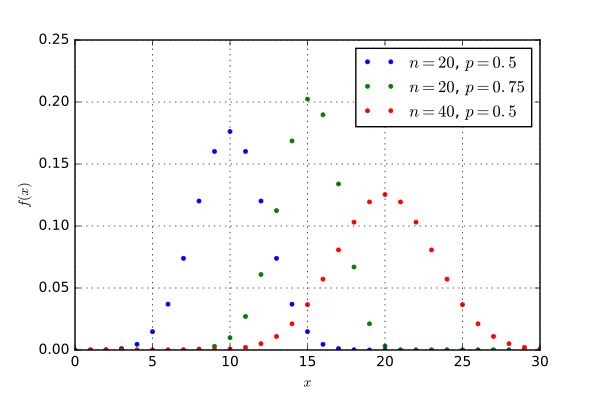
\includegraphics[width=\linewidth]{./img/binom.png}
		\caption*{а) биномиальное распределение.}
	\end{minipage}
	\noindent
	\begin{minipage}[t]{.45\textwidth}
		\centering
		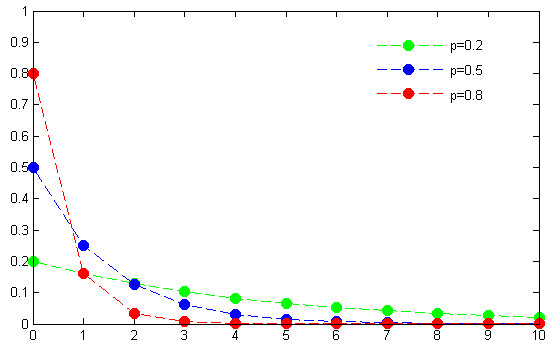
\includegraphics[width=\linewidth]{./img/geom.jpg}
		\caption*{б) геометрическое распределение.}
	\end{minipage}
	\begin{minipage}[t]{.45\textwidth}
		\centering
		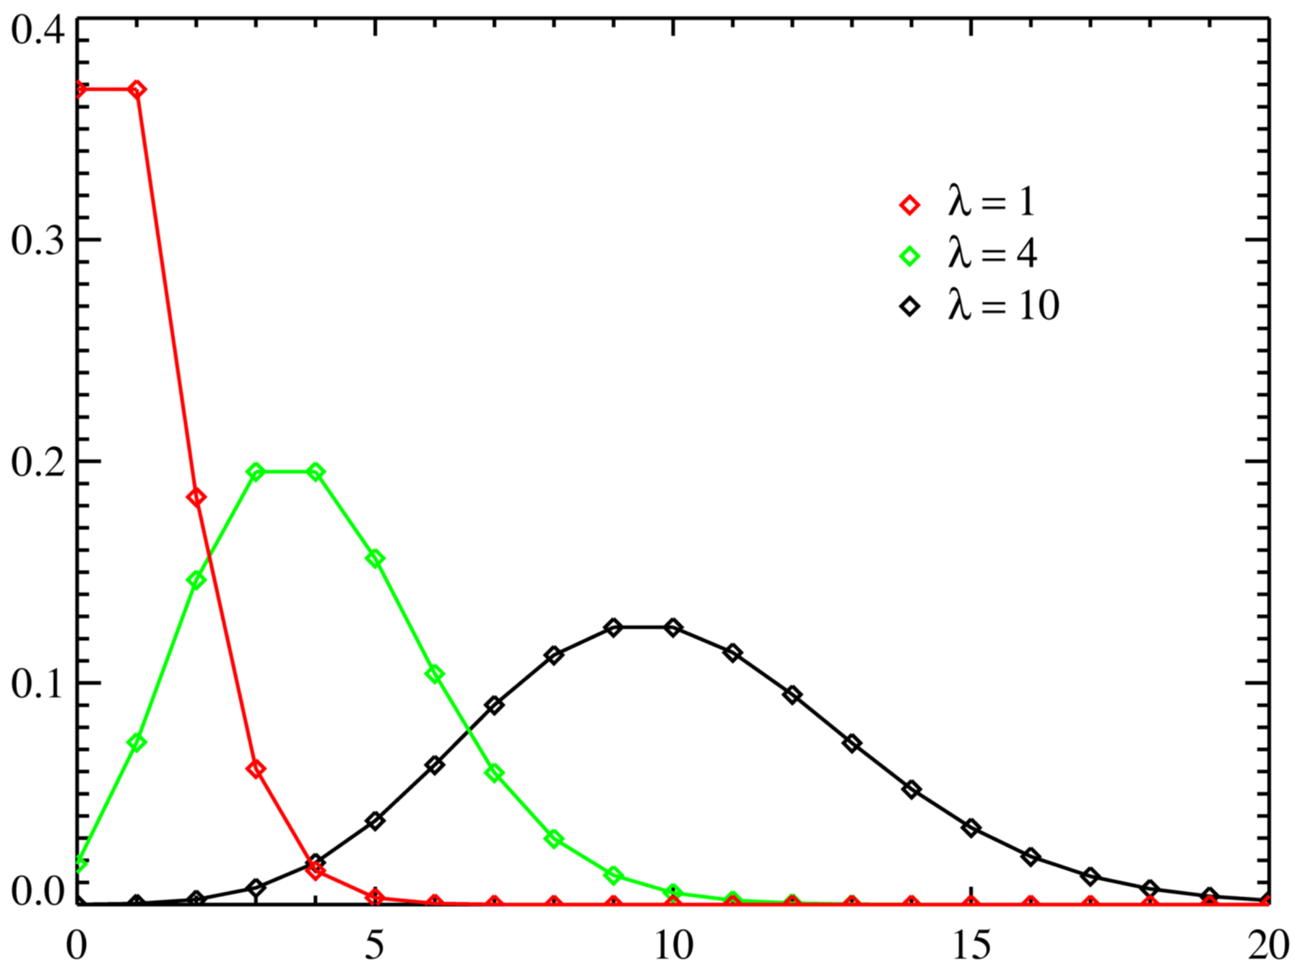
\includegraphics[width=\linewidth]{./img/poisson.png}
		\caption*{в) распределение Пуассона.}
	\end{minipage}
	\caption{Графики дискретных вероятностных распределений.}
	\label{fig:distr_1}
\end{figure}

\begin{figure}[H]
	\centering
	\begin{minipage}[t]{.45\textwidth}
		\centering
		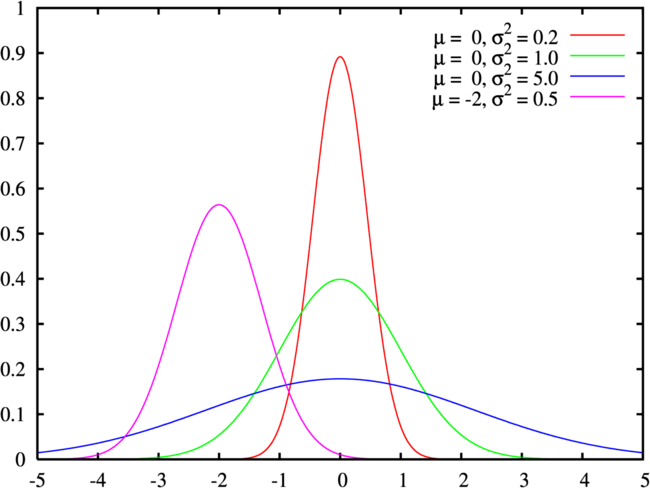
\includegraphics[width=\linewidth]{./img/norm.png}
		\caption*{а) нормальное распределение.}
	\end{minipage}
	\noindent
	\begin{minipage}[t]{.45\textwidth}
		\centering
		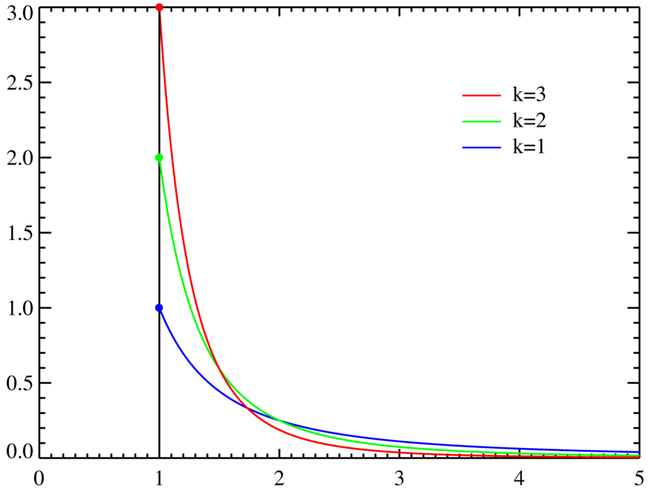
\includegraphics[width=\linewidth]{./img/paretto.png}
		\caption*{б) распределение Парето.}
	\end{minipage}
	\begin{minipage}[t]{.45\textwidth}
		\centering
		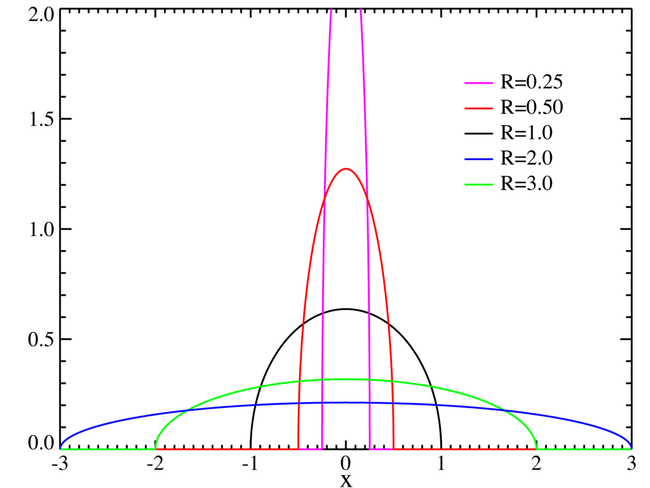
\includegraphics[width=\linewidth]{./img/vigner.png}
		\caption*{в) полукруговое распределение Вигнера.}
	\end{minipage}
	\caption{Графики непрерывных вероятностных распределений.}
	\label{fig:distr_2}
\end{figure}

%%%%%%%%%%%%%%%%%%%%%%%%%%%%%% машинное обучение %%%%%%%%%%%%%%%%%%%%%%%%%%%%%%%
\subsection{Машинное обучение}
Машинное обучение -- это раздел информатики, который посвящён созданию алгоритмов, опирающихся на набор данных о каком-либо явлении, причём эти данные могут быть различного происхождения: получены из окружающей среды, порождены другими алгоритмами или созданы вручную\cite{ml1}.

Моделью машинного обучения называют алгоритм или набор алгоритмов, которые обучаются на большом количестве данных с целью выявить закономерности для дальнейших прогнозов на аналогичных данных.

В машинном обучении выделяют несколько ключевых направлений: 

\begin{enumerate}
    \item Классическое машинное обучение, состоящее из определённого набора алгоритмов, которые во многих случаях можно легко интерпретировать, что крайне полезно, если модель используется для решения задач бизнеса;
    \item Глубокое обучение, подразделами которого выделяют: компьютерное зрение, языковые модели и нейронные сети в общем случае.
\end{enumerate}

Кроме того, машинное обучение можно классифицировать по типу обучения, выделяя три основных подхода:
\begin{enumerate}
    \item Обучение с учителем -- это вид обучения, при котором алгоритм машинного обучения, в дальнейшем -- модель, обучается на основе размеченных данных, то есть для каждого объекта в тренировочном наборе уже известен правильный ответ, который модель должна предсказать. Это наиболее распространённый тип обучения, применяемый в задачах, где необходимо поставить объект в соответствие некоторой группе -- классу;
    \item Обучение без учителя -- это вид обучения, при котором модель учится решать задачи без размеченных данных, то есть ответ задачи заранее неизвестен, ярким примером задачи такого типа является кластеризация, то есть разбиение множества объектов на непересекающиеся подмножества -- кластеры (англ. cluster);
    \item Обучение с подкреплением -- это вид обучения, при котором модель так же как и в обучении с учителем не имеет примеров, однако за «свой выбор» она получает «поощрение» или «наказание», после чего перестраивается, чтобы больше не получать «наказаний».
\end{enumerate}

Классификация объектов на изображениях с использованием алгоритмических методов является сложной задачей, поскольку для её эффективного решения требуются специальные подходы, позволяющие точно идентифицировать объекты, расположенные на изображении. Когда человек классифицирует объект, он, как правило, не использует чётко заданный алгоритм, а опирается на свой опыт, знания и интуицию, что является формально не определяемым понятием.

Для того, чтобы приблизиться к имитации мыслительного процесса человека, в том числе, классификации им объектов, учёные занялись изучением нейронных сетей в его мозге, что в дальнейшем привело к созданию искусственных нейронных сетей (далее -- нейронных сетей), которые способны учиться и принимать решения на основе большого количества входных данных.

Обучение нейронных сетей заключается в оптимизации весов нейронов, то есть параметров, определяющих взаимодействие между элементами искусственной нейронной сети, таким образом, чтобы нейронная сеть могла решать поставленную задачу с заранее определённой точностью.

%%%%%%%%%%%%%%%%%%%%%%%%%%%%%% компьютерное зрение %%%%%%%%%%%%%%%%%%%%%%%%%%%%%%%
\subsection{Компьютерное зрение}
Особое место в области машинного обучения, а конкретнее -- в области глубокого обучения, занимает компьютерное зрение. Данное направление занимается исследованиями в области различного рода обработки изображений\cite{cv1}.

Среди главных задач компьютерного зрения можно выделить:
\begin{enumerate}
    \item Распознавание объектов -- идентификация и классификация объектов на изображении, таких как лица, текст, предметы и другие объекты;
    \item Сегментация изображений -- разделение изображения на несколько областей, каждая из которых соответствует отдельному объекту. Сегментация может быть выполнена на основе различных признаков, таких как цвет, форма или класс объектов;
    \item Стилизация изображений -- применение различных фильтров для изменения текстуры изображения, например: превращение фотографии в картину в стиле конкретного художника.
\end{enumerate}

Сложность задач компьютерного зрения связана с многообразием изображений и их вариативностью, это связано с несколькими факторами: камеры обладают разными разрешениями, фотографии делаются в разное время и под разными углами, также, при съёмке на мобильный телефон может быть выбран специальный фильтр, который сделает фотографию ещё более сложной и уникальной. 

Современные методы в области компьютерного зрения активно используют искусственные нейронные сети (далее -- нейронные сети), в основном -- свёрточные нейронные сети (англ. CNN), которые позволяют извлекать нетривиальные признаки из изображений и обрабатывать их для получения полезной информации относительно быстро и эффективно. Свёрточные нейронные сети состоят из нескольких слоёв, выполняющих операции свёртки и нелинейных преобразований, подробнее о понятии «свёртка» будет сказано в следующей части. 

Хоть нейронные сети и являются мощным инструментом при решении задач в области компьютерного зрения, однако при разработке и обучении нейронных сетей с большим количеством слоёв и входных параметров, необходимо проявлять осторожность, поскольку существует риск переобучения. В случае переобучения нейронная сеть может «обращать внимание» на несущественные особенности изображения, такое поведение приведет к высокому показателю точности на тренировочных данных, но плохой обобщающей способности при обработке новых данных, то есть приведёт к явлению, которое называется переобучением.

Для предотвращения переобучения разработаны различные методы. Некоторые из них направлены на улучшение архитектуры нейронной сети, другие же фокусируются на обработке входных данных, таких как искусственное увеличение объёма данных за счёт преобразований изображения, такая техника называется аугментацией данных (англ. data augmentation), она позволяет нейронной сети быть более устойчивой и универсальной при работе с разнообразными входными изображениями.

%%%%%%%%%%%%%%%%%%%%%%%%%%%%%% преобразование изображений %%%%%%%%%%%%%%%%%%%%%%%%%%%%%%%
\subsection{Изображения}

\subsubsection{Тензорное представление изображений}
Если рассматривать изображения как объекты для обработки алгоритмами компьютерного зрения, можно сказать, что они представляют собой упорядоченный набор пикселей. Каждый пиксель -- это вектор, для чёрно-белых изображений он состоит из одного канала, а для цветных — из трёх: интенсивностей красного, зелёного и синего цветов\cite{yandex}.

Интенсивность каждого канала описывается числом в диапазоне от 0 до 1, но на практике этот интервал дискретизируется до значений от 0 до 255, что соответствует восьмибитной точности. Нулевая интенсивность по всем трём компонентам (0, 0, 0) соответствует чёрному цвету, в то время как максимальная интенсивность -- (255, 255, 255) соответствует белому цвету.

Таким образом, когда человек видит на экране компьютера цветное изображение, то на самом деле это изображение является векторами из пикселей с заданными интенсивностями, уложенными в ряд определённым образом. Длина такого вектора называется шириной изображения W, а количество векторов уложенных в ряд -- высотой изображения H. То есть, изображение можно рассматривать как тензор HxWx3, состоящий из чисел от 0 до 255.

Описанное представление отражено на рисунке \ref{fig:tensor}, который взят из ресурса\cite{yandex}.
\begin{figure}[H]
	\centering
	\begin{minipage}[t]{.5\textwidth}
		\centering
		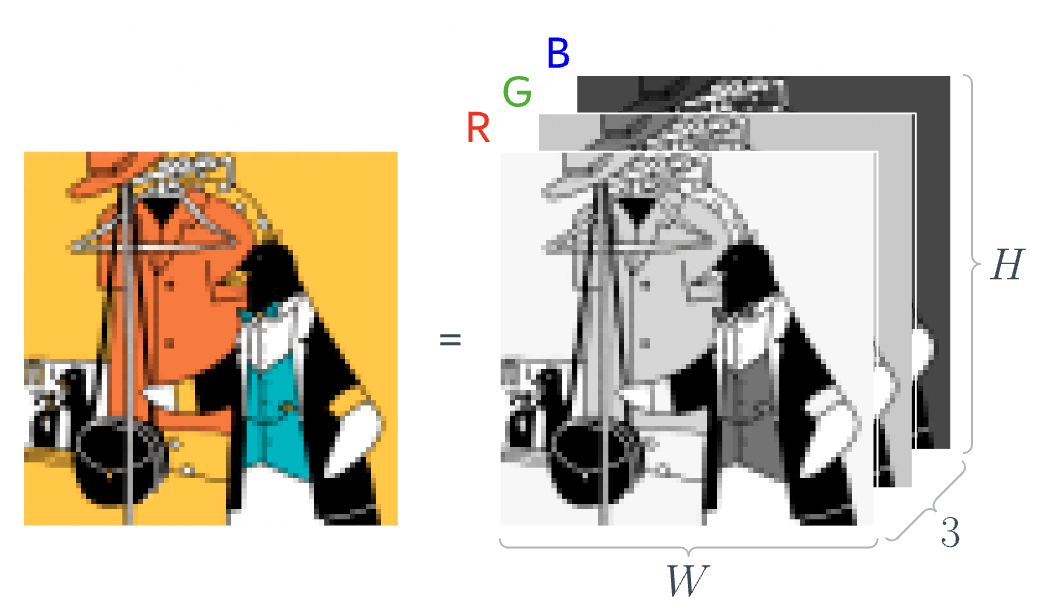
\includegraphics[width=\linewidth]{./img/tensor.png}
	\end{minipage}
	\caption{Представление изображения в виде тензора.}
	\label{fig:tensor}
\end{figure}

\subsubsection{Обработка изображений нейронной сетью}
Самым простым методом для построения нейронной сети с целью классификации изображений является следующий: рассмотреть изображение как тензор, после чего растянуть полученный тензор в длинный одномерный вектор и использовать обычную многослойную нейронную сеть. Однако данный подход имеет ряд существенных недостатков.

Во-первых, полученный одномерный вектор имеет большую длину, что значительно увеличит время его обработки многослойной нейронной сетью, на вход которой он будет подаваться.

Во-вторых, и это особенно важно, при растягивании тензора теряются пространственные связи между векторами, задающими изображение. Эти связи могли содержать ключевую информацию, которую нейронная сеть должна была выявить для успешного решения поставленной задачи, например классификации.

\subsubsection{Операции над изображением в свёрточных нейронных сетях}
Для решения проблем, связанных с растягиванием тензора, который является численным представлением изображения, в длинный вектор, в нейронных сетях используют операцию свёртки (англ. convolution) и объединения (англ. pooling), на практике распространён метод под названием max pooling\cite{itmo}. 

Свёртка представляет собой операцию над парой матриц $A_{n_x*n_y}$ и $B_{m_x*m_y}$, результатом которой является матрица $C_{(n_x-m_x+1)*(n_y-m_y+1)}$, элементы которой определяются по формуле \ref{eq:formul}

\begin{equation}\label{eq:formul}
	C_{i,j} = \sum_{u=0}^{m_x-1} \sum_{v=0}^{m_y-1} A_{i+u,j+v} B_{u,v}
\end{equation}

Данную формулу можно трактовать так: матрица $B_{m_x*m_y}$ «двигается» по матрице $A_{n_x*n_y}$, и в каждом её положении считается скалярное произведение матрицы $B_{m_x*m_y}$ и части матрицы $A_{n_x*n_y}$, над которой она оказалась. Визуализация данного процесса представлена на рисунке \ref{fig:svertka}, взятом с ресурса\cite{itmo}.

\begin{figure}[H]
	\centering
	\begin{minipage}[t]{.5\textwidth}
		\centering
		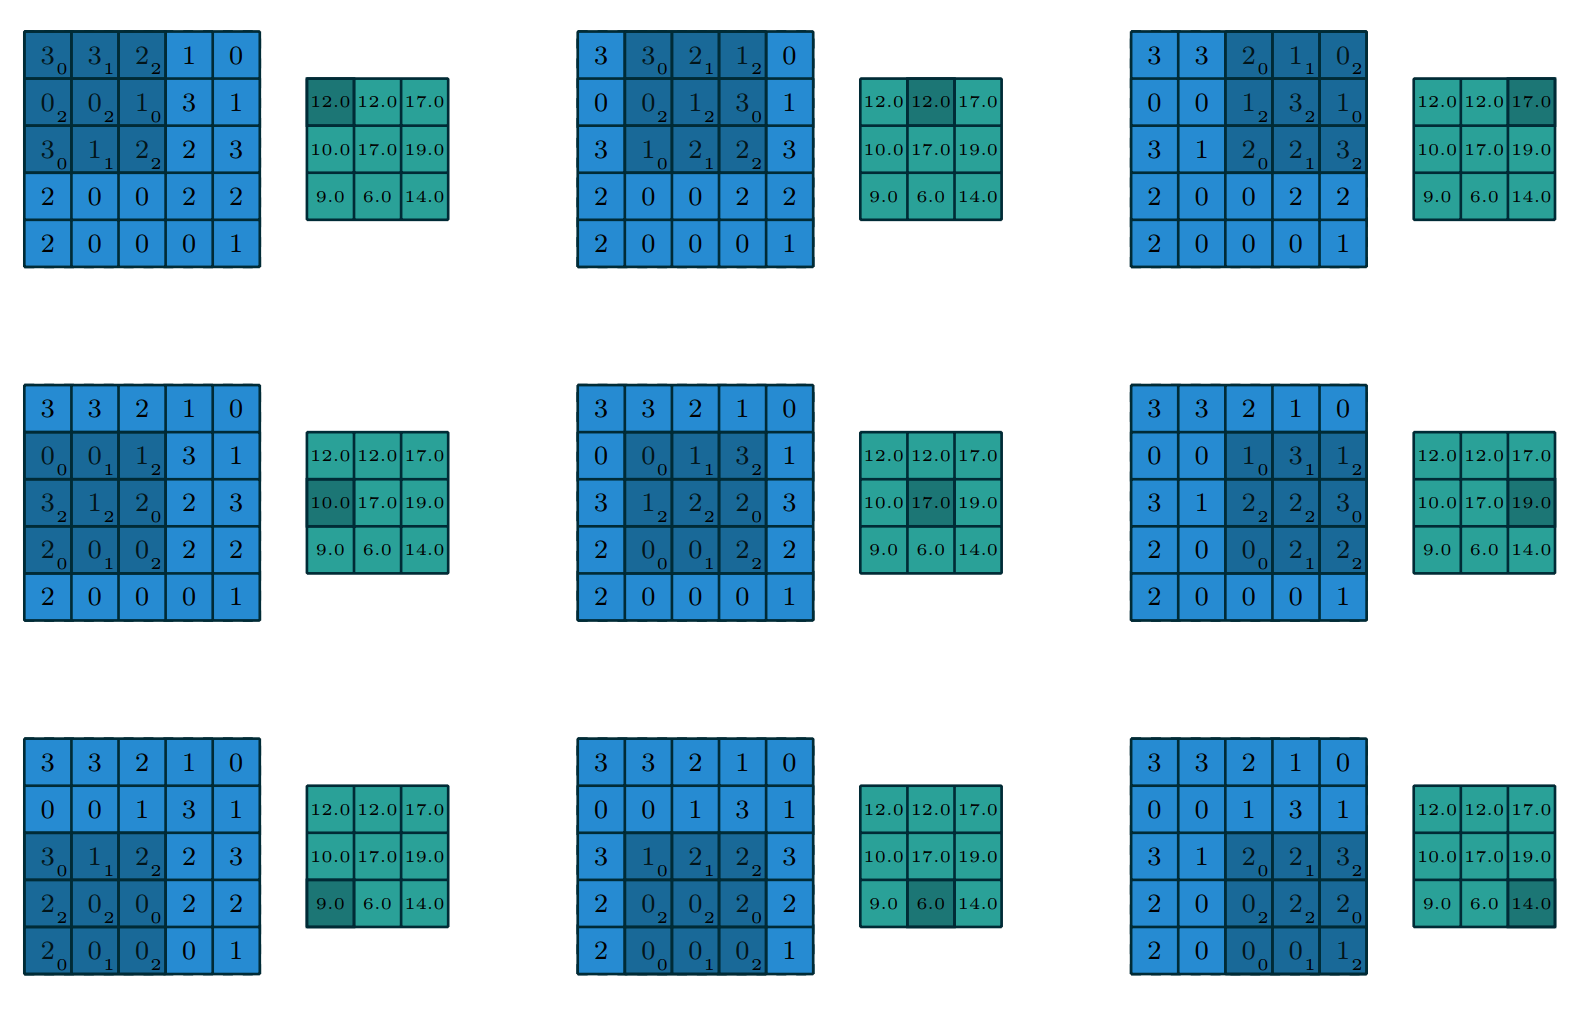
\includegraphics[width=\linewidth]{./img/svertka.png}
	\end{minipage}
	\caption{Пример процесса свёртки.}
	\label{fig:svertka}
\end{figure}

Max pooling -- это метод объединения, который снижает размерность данных после свёртки, выбирая максимальное значение из небольших областей изображения. Таким образом, он уменьшает объём информации, которую нужно обработать, и делает нейронную сеть более устойчивой к смещениям объектов на изображении. Визуализация данного метода представлена на рисунке \ref{fig:maxpooling}, взятом с ресурса\cite{itmo}.

\begin{figure}[H]
	\centering
	\begin{minipage}[t]{.5\textwidth}
		\centering
		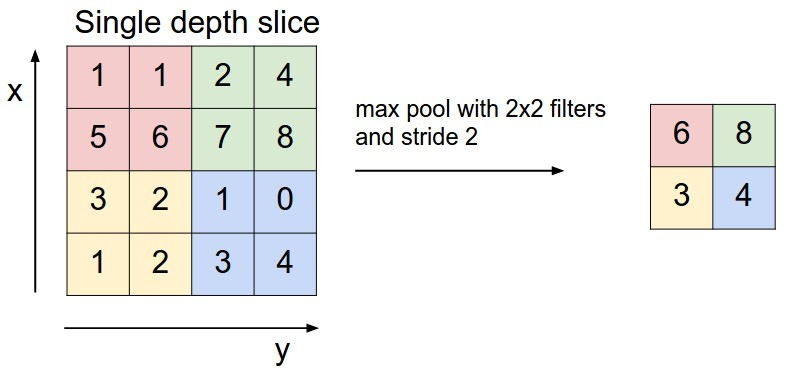
\includegraphics[width=\linewidth]{./img/maxpooling.jpeg}
	\end{minipage}
	\caption{Пример метода Max pooling.}
	\label{fig:maxpooling}
\end{figure}

Данные методы позволяют сохранить пространственные связи между пикселями изображения, а также сократить размер данных, что ускоряет процесс обучения без потери качества, поэтому они являются основными блоками при построении свёрточных нейронных сетей.

\subsubsection{Преобразования изображений}
Над изображениями также можно производить различные преобразования, в данной курсовой работе рассматриваются три типа преобразований изображений: изменение их свойств (яркости, контрастности и насыщенности), перспективное преобразование и поворот.

Данные преобразования можно описать через манипуляции, проводящиеся над пикселями. Изменение свойств изображения, таких как яркость, контрастность и насыщенность, связано с изменением значений интенсивности каждого пикселя. Перспективное преобразование предполагает перемещение пикселей на новые позиции, создавая эффект наклона, сжатия или растяжения изображения. Поворот изменяет расположение пикселей так, чтобы изображение было повернуто вокруг заданной точки на определённый угол, сохраняя при этом его структуру.

Примеры преобразований, которые были применены к изображениям в данной курсовой работе, представлены на рисунке \ref{fig:transforms}.

\begin{figure}[H]
	\centering
	\begin{minipage}[t]{.3\textwidth}
		\centering
		
\includegraphics[width=\linewidth]{./img/perspec.png}
		\caption*{а) перспективное преобразование.}
	\end{minipage}
	\noindent
	\begin{minipage}[t]{.3\textwidth}
		\centering
		
\includegraphics[width=\linewidth]{./img/rotate.png}
		\caption*{б) поворот.}
	\end{minipage}
	\begin{minipage}[t]{.3\textwidth}
		\centering
		
\includegraphics[width=\linewidth]{./img/color.png}
		\caption*{в) изменение свойств изображения.}
	\end{minipage}
	\caption{Пример преобразований изображения перед обучением.}
	\label{fig:transforms}
\end{figure}

%%%%%%%%%%%%%%%%%%%%%%%%%%%%%%%%% РАЗРАБОТКА %%%%%%%%%%%%%%%%%%%%%%%%%%%%%%%%%
\section{Разработка приложения}
Модель машинного обучения должна выполнять классификацию графиков вероятностных распределений следующих типов:
\begin{enumerate} 
    \item биномиальное распределение;
    \item геометрическое распределение;
    \item распределение Пуассона;
    \item нормальное распределение;
    \item распределение Парето;
    \item полукруговое распределение Вигнера.
\end{enumerate}

Для достижения высокой точности классификации планируется провести исследование, включающее разработку трёх свёрточных нейронных сетей. Эти нейронные сети будут обучены на изображениях графиков вероятностных функций, подвергнутых различным типам аугментаций. После обучения для каждой нейронной сети будут рассчитаны метрики качества: точность классификации и значение функции потерь. На основе полученных результатов будет выбрана лучшая.

Проект включает две основные части:
\begin{enumerate} 
    \item Подготовку данных -- изображений графиков вероятностных функций;
    \item Реализацию, обучение и анализ моделей машинного обучения с оценкой их метрик качества для выбора наиболее эффективной модели.
\end{enumerate}

%%%%%%%%%%%%%%%%%%%%%%%%%%%%% архитектура подготовки данных %%%%%%%%%%%%%%%%%%%%%%%%%%%%
\subsection{Архитектура модуля подготовки данных}
Модуль подготовки данных играет ключевую роль в построении модели, так как качество данных, на которых будет происходить обучение, непосредственно влияет на способность нейронной сети эффективно классифицировать изображения графиков вероятностных распределений. После долгих поисков нужного набора данных для тренировки, было принято решение генерировать изображения самостоятельно. 

В связи с этими особенностями, модуль с генерацией нужных данных включает в себя:
\begin{itemize}
    \item Порождение графиков вероятностных распределений с использованием специальной библиотеки для работы со статистическими функциями. Это позволяет задавать параметры распределений и создавать различные варианты графиков. Для визуализации функциональных зависимостей используется библиотека для построения графиков;
    \item Визуализацию графиков вероятностных распределений, полученных на предыдущем шаге;
    \item Сохранение сгенерированных графиков в заданной директории с последующим архивированием данных в формате .zip.
\end{itemize}

%%%%%%%%%%%%%%%%%%%%%%%%%%%%% архитектура подготовки данных %%%%%%%%%%%%%%%%%%%%%%%%%%%%
\subsection{Архитектура модуля разработки нейронной сети}
Для того, чтобы свёрточная нейронная сеть давала прогнозы осмысленно, необходимо обучить её на данных, то есть показать примеры изображений, а также предоставить метку-ответ, с которой в последствии будет сопоставлен прогноз модели. Для обучения необходим специальный формат входных данных. Само обучение происходит эпохами, где эпохой называют один просмотр нейронной сетью всей тренировочной выборки. Для достижения высокой точности классификации требуется несколько эпох, так как с каждой из них нейронная сеть извлекает всё больше информации об объекте, что способствует её обобщающим возможностям.

Модуль разработки и обучения модели состоит из следующих компонентов: 
\begin{itemize}
    \item Подготовка данных для обучения и валидации: применение аугментаций для изображений графиков вероятностных распределений, преобразование изображений в специальный формат, необходимый для работы нейронной сети, а именно -- преобразование изображений в тензоры, задание размеров изображений. Реализация класса \verb|Dataset| для удобного представления данных и подготовки их к обучению, а также объекта \verb|DataLoader| для совместимости с входами нейронной сети и организации процесса подачи данных в ходе тренировки и тестирования;
    \item Конструирование класса нейронной сети, описание её внутреннего устройства и необходимых для обучения методов. Реализация функций для обучения на одной эпохе, а также полного цикла работы модели, включающего обучение и валидацию в течение нескольких эпох. Подсчёт ключевых метрик -- точности и значения функции потерь на каждой эпохе;
    \item Визуализация результатов: создание функций для графического представления метрик, собранных в процессе обучения и валидации, а также функции для отображения изображений из обучающей и тестовой выборок. 
\end{itemize}

%%%%%%%%%%%%%%%%%%%%%%%%%%%% выбор инструментов разработки %%%%%%%%%%%%%%%%%%%%%%%%%%%
\subsection{Выбор инструментов разработки}

Для реализации проекта был выбран язык программирования \verb|Python|\cite{python}. Этот выбор обусловлен рядом факторов:
\begin{enumerate} 
    \item \verb|Python| предоставляет широкий набор библиотек для работы со статистикой (вычисление функции плотности, порождение распределений, подсчёт статистических характеристик и другое), визуализацией графиков (столбчатая диаграмма, круговая диаграмма, график функциональных зависимостей), манипулирования математическими объектами: матрицами, векторами, градиентами и другими; 
    \item Развитая экосистема для построения моделей машинного обучения. Большинство библиотек, используемых для разработки, обучения и тестирования моделей машинного обучения написаны на \verb|Python|. Это делает его наиболее подходящим языком для задач, связанных с данной курсовой работы;
    \item Доступность обучающих материалов. \verb|Python| является одним из самых популярных языков программирования, благодаря чему существует множество учебных ресурсов и примеров использования различных библиотек, которые активно используют и развивают специалисты в области машинного обучения;
    \item Удобство и простота использования. \verb|Python| имеет интуитивно понятный синтаксис, благодаря чему значительно ускоряется процесс разработки.
\end{enumerate}

Подробнее остановимся на библиотеках, которые были использованы при реализации данного проекта, в целом, их можно разделить на три класса.

\begin{enumerate} 
    \item Библиотеки для работы с нейронными сетями обеспечивающие построение, валидацию, оптимизацию обучения нейронной сети, а также работу с математическими объектами, такими как векторы предсказаний и тензоры, представляющие изображения:                
        \begin{itemize} 
            \item \verb|NumPy|\cite{numpy} -- библиотека, предоставляющая широкий набор математических функций для работы с массивами, векторами и тензорами;
            \item \verb|PyTorch|\cite{pytorch} -- библиотека, включающая функции для создания и обучения нейронных сетей, преобразования данных в формат, совместимый с моделью, а также методы для оптимизации и расчёта функций ошибки;
            \item \verb|torchvision|\cite{torchvision} -- библиотека, ориентированная на задачи компьютерного зрения. Она содержит функции для обработки изображений, а также реализации различных видов аугментаций.
        \end{itemize}
    \item Библиотеки для визуализации, а именно для построения графиков метрик, отображения изображений и анализа времени выполнения: 
        \begin{itemize} 
            \item \verb|Matplotlib|\cite{matplot} -- библиотека для построения различных типов графиков, таких как линейные, столбчатые, круговые и другие;
            \item \verb|IPython|\cite{ipython} -- библиотека, упрощающая взаимодействие с пользователем. Она поддерживает подсветку синтаксиса, логирование, а также обеспечивает очищение буфера после отображения результатов;
            \item \verb|tqdm|\cite{tqdm} -- библиотека, предоставляющая индикаторы выполнения, позволяющие отслеживать прогресс выполнения команд, функций или циклов.
        \end{itemize}
    \item Вспомогательные библиотеки
        \begin{itemize} 
            \item \verb|SciPy|\cite{scipy} -- библиотека для анализа данных, построения вероятностных моделей и работы с большими массивами информации. В частности, она включает в себя статистические функции;
            \item \verb|shutil|\cite{shutil} -- библиотека для выполнения операций с файлами, включая их перемещение, копирование или удаление;
            \item \verb|google|\cite{google} -- библиотека, предоставляющая доступ к сервисам \verb|Google|. С её помощью можно, например, подключаться к\verb|Google| диску или\verb|Google| таблицам напрямую из кода.
        \end{itemize}
\end{enumerate}

%%%%%%%%%%%%%%%%%%%%%%%%%%%%%%%%% РЕАЛИЗАЦИЯ %%%%%%%%%%%%%%%%%%%%%%%%%%%%%%%%%
\section{Реализация приложения}

Для выполнения поставленной задачи необходимо реализовать два модуля. Первый модуль будет отвечать за генерацию данных, а второй — за предварительную обработку изображений (препроцессинг), их преобразование в необходимый формат и интеграцию с нейронной сетью для корректной обработки входных данных.

В качестве среды разработки для данного проекта была выбрана облачная платформа \verb|Google Colab|\cite{colab}, предназначенная для исследовательских задач в области машинного обучения и анализа данных.

Данная среда была выбрана по ряду причин: 
\begin{enumerate}
    \item Совместима с языком программирования \verb|Python|;
    \item Является бесплатной и предоставляет доступ к вычислительным ресурсам, включая \verb|GPU|, что позволяет обучать довольно сложные и объёмные архитектуры нейронных сетей, не имея мощного домашнего оборудования;
    \item Возможность запускать ячейки с кодом с мобильных устройств, что обеспечивает удобство работы в условиях отсутствия компьютера;
    \item Поддержка интеграции с сервисами \verb|Google|, такими как \verb|Google| диск. Это позволяет хранить данные и файлы в облачном хранилище, освобождая память локального устройства и обеспечивая удобный доступ к материалам при выполнении вычислений.
\end{enumerate}

%%%%%%%%%%%%%%%%%%%%%%%%%% особенности реализации генерации даных %%%%%%%%%%%%%%%%%%%%%%%%%%%

\subsection{Особенности реализации модуля генерации данных}
Для реализации модуля генерации графиков функций вероятностных распределений был создан \verb|Google Colab Notebook| (далее блокнот для разработки). Помимо основной функциональности, в данном блокноте были приведены теоретические сведения из статистики и теории вероятностей, которые используются в проекте.

\begin{enumerate} 
    \item Для генерации графиков использовался модуль \verb|stats| библиотеки \verb|scipy|. Параметры для каждого распределения задавались произвольным образом, что позволило создать разнообразные графики. Данный подход обеспечил возможность обучения модели на данных, которые имеют общие признаки, вместо запоминания полностью одинаковых изображений;
    \item Для обучения модели требовалось большое количество данных. В рамках реализации было создано по тысяче графиков для каждого типа распределения. В процессе генерации использовалась функция \verb|save_plot|, код которой представлен на листинге \ref{lst:saveplot}, которая выполняла отрисовку графика и сохраняла его в указанную директорию на \verb|Google| диске. Визуализация графиков включала в себя построение линий функций и заливку области под кривой (для непрерывных распределений). Добавление заливки необходимо, так как это позволяет снизить вычислительную сложность при классификации;
    \item После завершения генерации данных все изображения были архивированы с использованием библиотеки \verb|shutil|. Архивирование позволяет сократить занимаемое пространство и упростить дальнейшее использование сгенерированных данных. Полученный архив был сохранён на \verb|Google| диске для последующей загрузки и работы.
\end{enumerate}

%%%%%%%%%%%%%%%%%%%%%%%%%%%% особенности реализации нейронной сети %%%%%%%%%%%%%%%%%%%%%%%%%%%
\subsection{Особенности реализации нейронной сети}

Несмотря на доступ к \verb|GPU| благодаря платформе \verb|Google Colab|, ограничения на время использования ресурсов привели к необходимости упрощения проекта. Вместо архитектуры свёрточной нейронной сети \verb|VGG-16|\cite{vgg16} была реализована более компактная архитектура -- \verb|VGG-11|\cite{vgg11}. Также объём набора данных для обучения был уменьшен до шести тысяч изображений вместо изначально запланированных шестидесяти тысяч.

\begin{enumerate} 
    \item Вначале архив со сгенерированными изображениями был распакован, и данные распределены по папкам в соотношении 70\% для обучения и 30\% для тестирования. Для этого использовался метод произвольного разделения \verb|shuffle| из библиотеки \verb|random|\cite{random}, реализация данного этапа представлена на листинге \ref{lst:shuffle};
    \item Реализована функция визуализации изображений из различных выборок данных -- \verb|show_image|. С её помощью можно оценивать качество изображений и их распределение перед обучением модели. Кроме того, были заданы преобразования над изображениями, включая аугментации с целью проведения исследования и выбора лучшей нейронной сети. Реализация данной функции представлена на листинге \ref{lst:show};
    \item Для подготовки данных был разработан класс \verb|dataset_statistic|, который хранит в себе:
    \begin{itemize}
        \item путь \verb|root_dir| к папке, в которой находятся изображения;
        \item трансформации \verb|transforms|, которые должны быть применены к изображениям;
        \item список файлов \verb|files|, которые находятся в папке;
        \item метод \verb|__len__(self)|, возвращающий количество изображений, которые хранит объект класса \verb|dataset_statistic|;
        \item метод \verb|__getitem__(self, index)|, возвращающий преобразованное изображение по индексу.
    \end{itemize}
    Для каждого вида аугментации определяется объекта класса \verb|DataLoader|, это итерируемый объект, который позволяет эффективно и гибко подавать порции данных в нейронную сеть. Код с описанием данного класса и примером объявления объекта \verb|DataLoader|, представлен на листинге \ref{lst:dataloader};

    \item Архитектура модели свёрточной нейронной сети была реализована в виде класса \verb|MOLI_Net|, приведённом на листингах \ref{lst:molinet} и \ref{lst:molinet2}. Логически нейронная сеть поделена на две части: автокодировщик (англ. encoder), не формально называемый «тушкой» модели, который преобразует входные данные в уменьшенное по размерности представление, и многоголовное внимание (англ. multi-head attention) -- архитектура, направленная на выявление связей между элементами полученных входных данных. Класс состоит из метода \verb|__init__(self, img_channels=3, num_classes=6)|, в котором задаётся структура свёрточной нейронной сети. 
    
    Часть автокодировщика нейронной сети задаётся слоями: \verb|Conv2d| -- свёрточный слой, который определяется:
    \begin{itemize}
        \item количеством входных каналов -- \verb|in_channels|;
        \item количеством выходных каналов -- \verb|out_channels|;
        \item ядром свёртки с размерами матрицы ядра свёртки \verb|kernel_size|;
        \item шаг, с которым ядро свёртки перемещается по матрице изображения -- \verb|stride|;
        \item дополнительный параметр для сохранения размера изображения после процедуры свёртки -- \verb|padding|.
    \end{itemize}
    После некоторых слоёв включён метод для нормализации данных -- \verb|BatchNorm2d|, а также \verb|MaxPool2d|. После каждого слоя к данным применяется нелинейная функция активации -- \verb|ReLU()|. 
    
    «Голова» нейронной сети задаётся тремя линейными слоями -- \verb|Linear|, после первых двух применена нелинейная функция активации -- \verb|ReLU()|, и метод \verb|Dropout(p=0.5)|, который работает в том случае, когда нейронная сеть находится в режиме обучения, данный метод отключает нейрон из сети с вероятностью равной 0.5. 
    
    Также в классе реализован метод \verb|forward|, который возвращает вектор, равный по длине количеству классов в нём, и на каждой позиции находится число -- вероятность принадлежности изображения к данному классу;

    \item Для обучения и валидации свёрточной нейронной сети реализованы функции: 
    \begin{itemize}
        \item \verb|train_epoch| -- функция обучения свёрточной нейронной сети, код которой представлен на листинге \ref{lst:trainepoch}.
        В данной функции нейронная сеть переключается в формат обучения методом \verb|model.train()|, далее, производится проход по выборке при помощи объекта класса \verb|DataLoader|, тензоры изображений и вектора меток их классов «сбрасываются» на \verb|GPU| для дальнейших вычислений. Производятся вычисления для определения класса, к которому принадлежит изображение, после чего считаются метрики: точность предсказаний и значение функции потерь, которые записываются в лог по средством специального сервиса -- \verb|Weights & Biases|\cite{wb}, а также возвращаются из функции через \verb|return|; 

        \item \verb|test| -- функция для тестирования свёрточной нейронной сети на выборке, которую она не видела при обучении, представлена на листинге \ref{lst:valepoch}. Данная функция аналогична по строению с \verb|train_epoch|, однако в начале нейронная сеть переключается в режим вычислений методом \verb|model.eval()|, а также, при подсчёте предсказаний модели, отключается автоматический подсчёт градиентов методом \verb|torch.no_grad()|;

        \item \verb|train| -- функция, производящая полный цикл обучения свёрточной нейронной сети, представлена на листинге \ref{lst:full}. В ней выполняется цикл по количеству эпох, в котором для каждой эпохи вышеописанными функциями считаются метрики точности и функции потерь с поправкой на размер порции данных (англ. batch), которые подаются модели. При итерации по каждой эпохе вызывается функция визуализации -- \verb|plot_logs|, которая отрисовывает значения метрик после обучения на текущей эпохе. Также в \verb|train| передаются значения метрик в сервис \verb|Weights & Biases|.
    \end{itemize}
\end{enumerate}

\subsection{Исследование преобразований изображений}
Для достижения высокой точности классификации было проведено исследование, которое включало в себя разработку трёх свёрточных нейронных сетей, которые были обучены на изображениях графиков вероятностных функций, подвергнутых различным типам аугментаций и одной свёрточной нейронной сети, которая обучалась на исходных изображениях.

\subsubsection{Подготовка к исследованию}
Преобразование над изображениями были выбраны следующие: 
\begin{itemize}
    \item Изменение свойств изображения: яркости, контрастности и насыщенности;
    \item Перспективное преобразование;
    \item Поворот.
\end{itemize}

Задание аугментаций, создание объекта класса \verb|Dataset| и \verb|DataLoader|, а также объявление нейронной сети представлены на листинге \ref{lst:test}.
Для того, чтобы проводить исследование, было принято решение использовать сервис для проведения анализа данных и опытов \verb|Weights & Biases|\cite{wb}, в него при обучении передавались данные логирования, а после конца обучения -- сохранялась модель в специальном формате .h5. Это позволит в дальнейшем загрузить лучшую, по меркам исследования, модель и использовать её в качестве основной решающей поставленную задачу. 

\subsubsection{Анализ логов}
На рисунке \ref{fig:logsbatch} приведены графики метрик (точность на тренировочной и валидационной выборках, значение функции потерь на тренировочной и валидационной выборках): нейронных сетей, обученных на изображениях: без аугментаций -- \verb|baseline|, с перспективным преобразованием -- \verb|perspective|, с поворотом -- \verb|rotate|, с изменением свойств изображения -- \verb|color|.

\begin{figure}[H]
	\centering
	\begin{minipage}[t]{.4\textwidth}
		\centering
		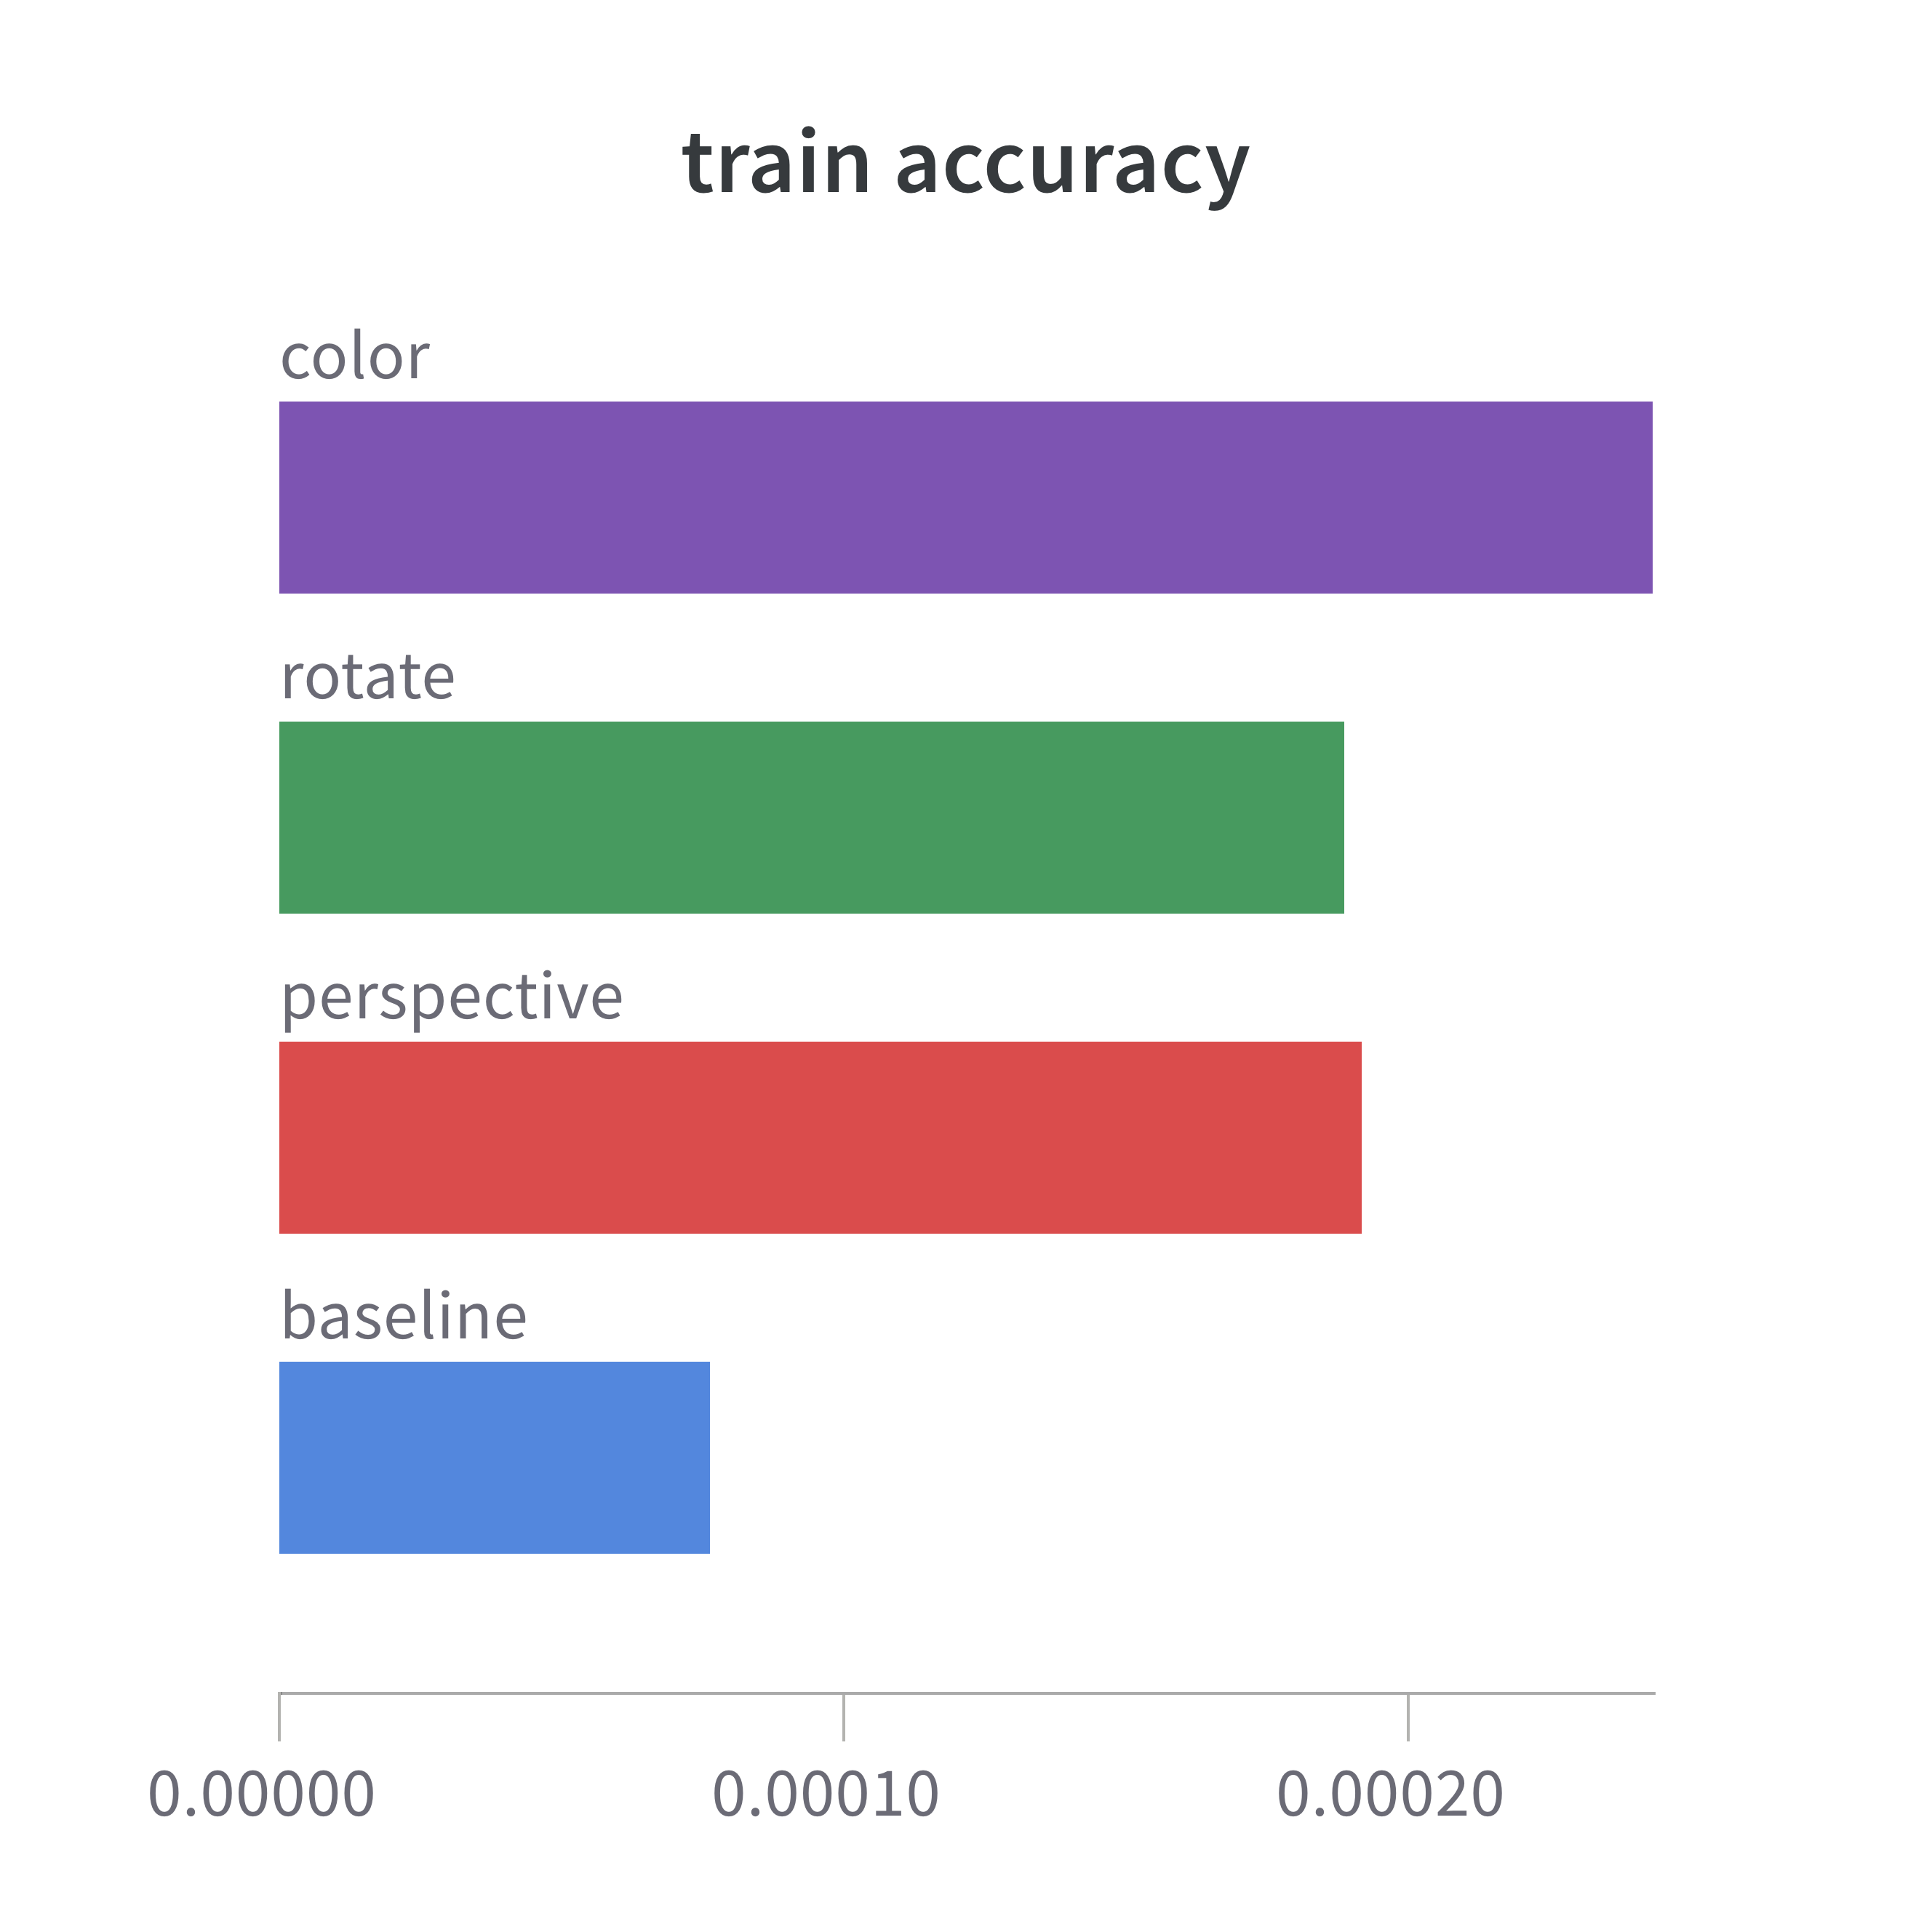
\includegraphics[width=0.75\textwidth]{./img/train_accuracy.png}
		\caption*{а) график метрики точности на тренировочной выборке.}
	\end{minipage}
        \begin{minipage}[t]{.4\linewidth}
		\centering
		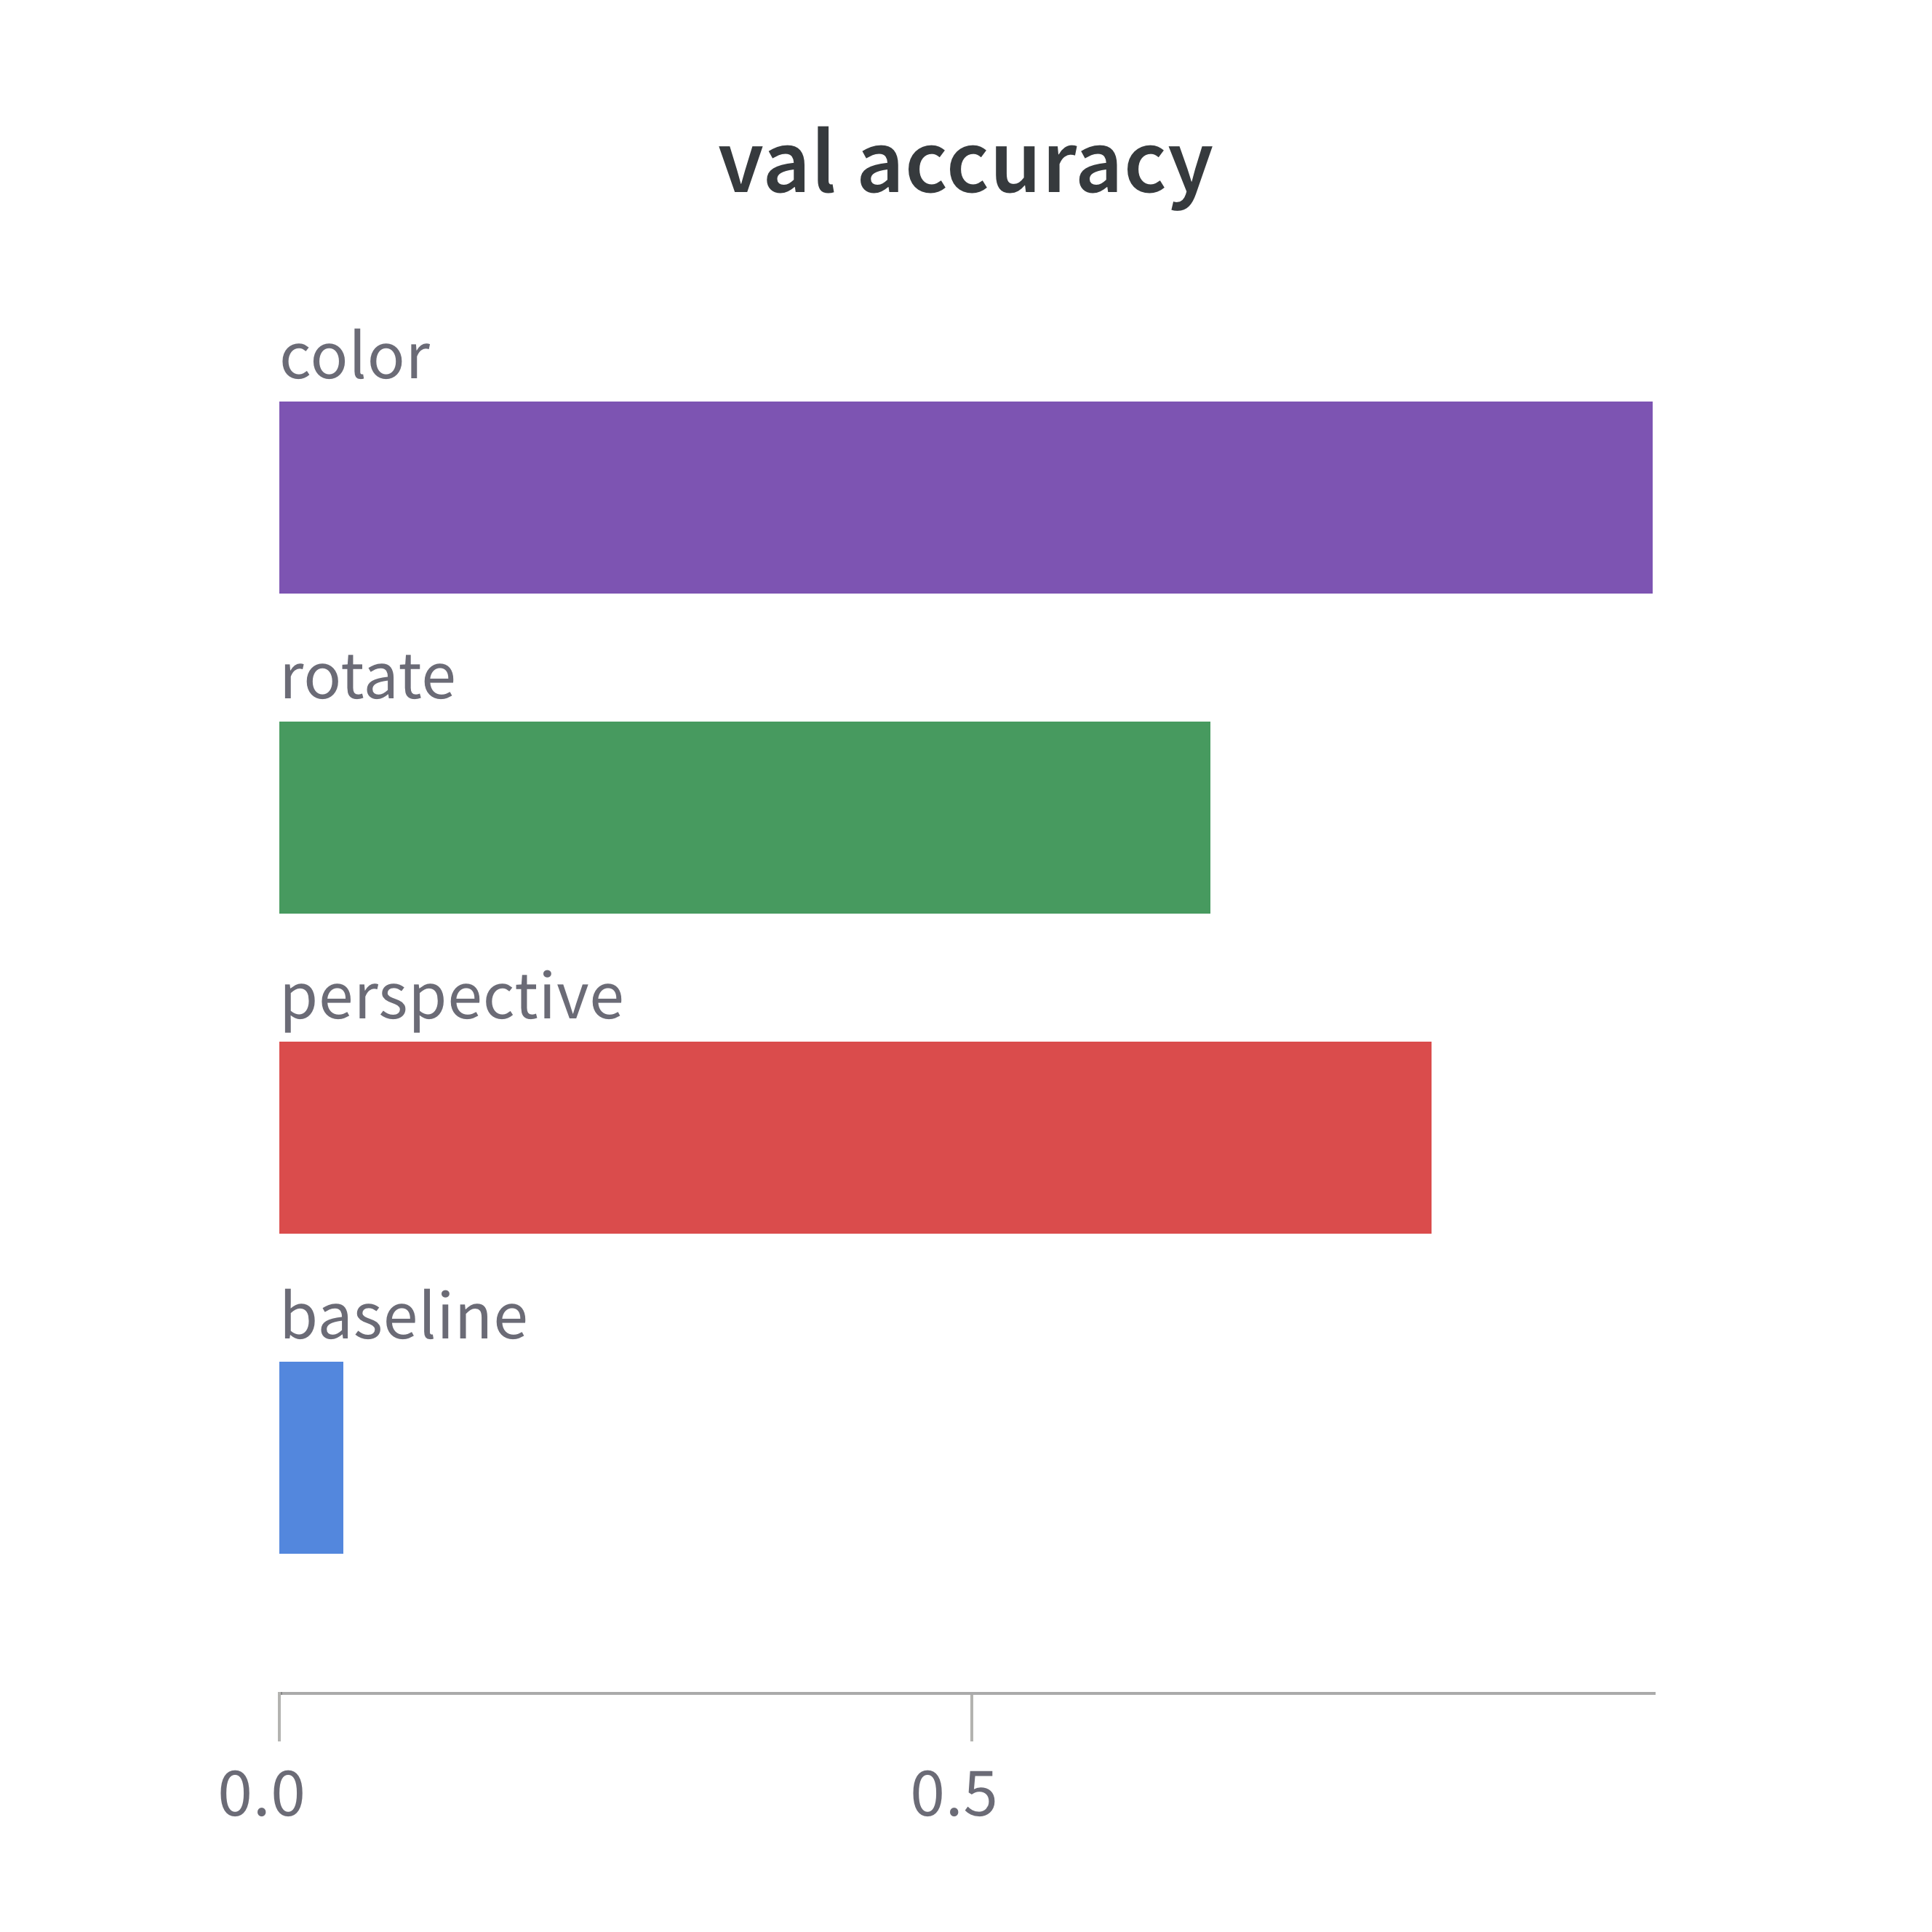
\includegraphics[width=0.75\textwidth]{./img/val_accuracy.png}
		\caption*{б) график метрики точности на валидационной выборке.}
	\end{minipage}
	\noindent
	\begin{minipage}[t]{.4\linewidth}
		\centering
		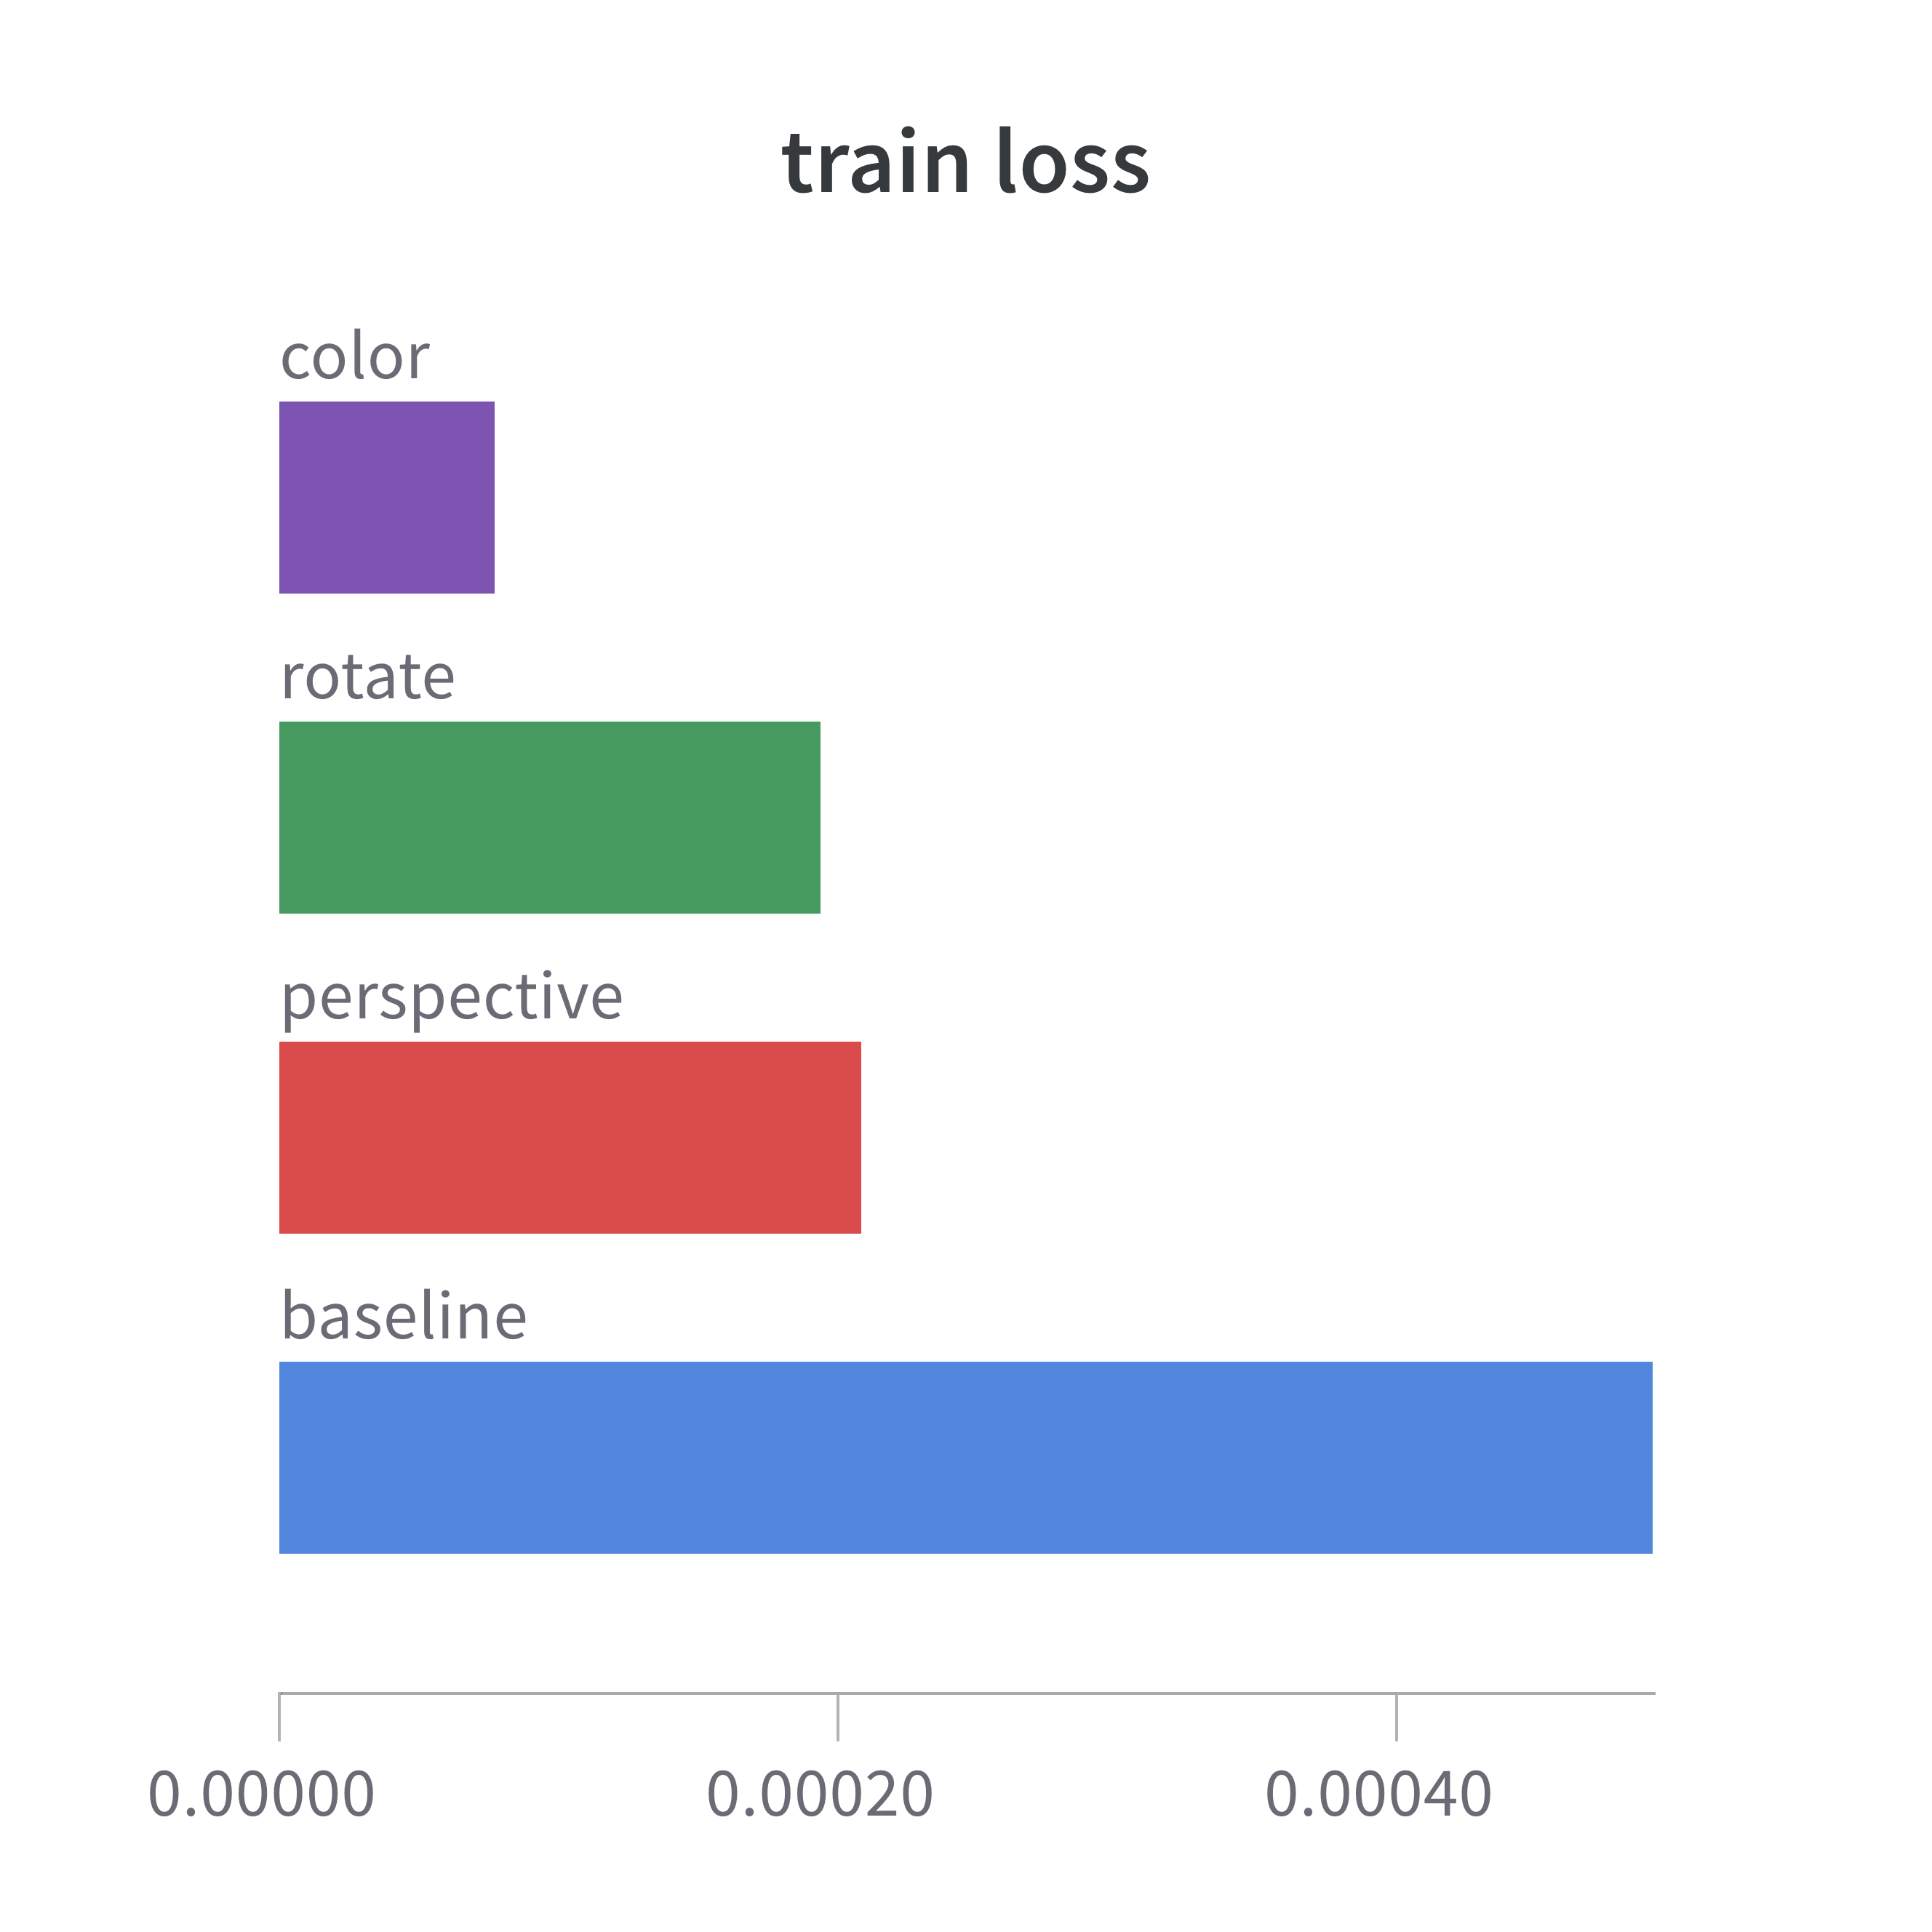
\includegraphics[width=0.75\textwidth]{./img/train_loss.png}
		\caption*{в) график значения функции потерь на тренировочной выборке.}
	\end{minipage}
	\begin{minipage}[t]{.4\textwidth}
		\centering
		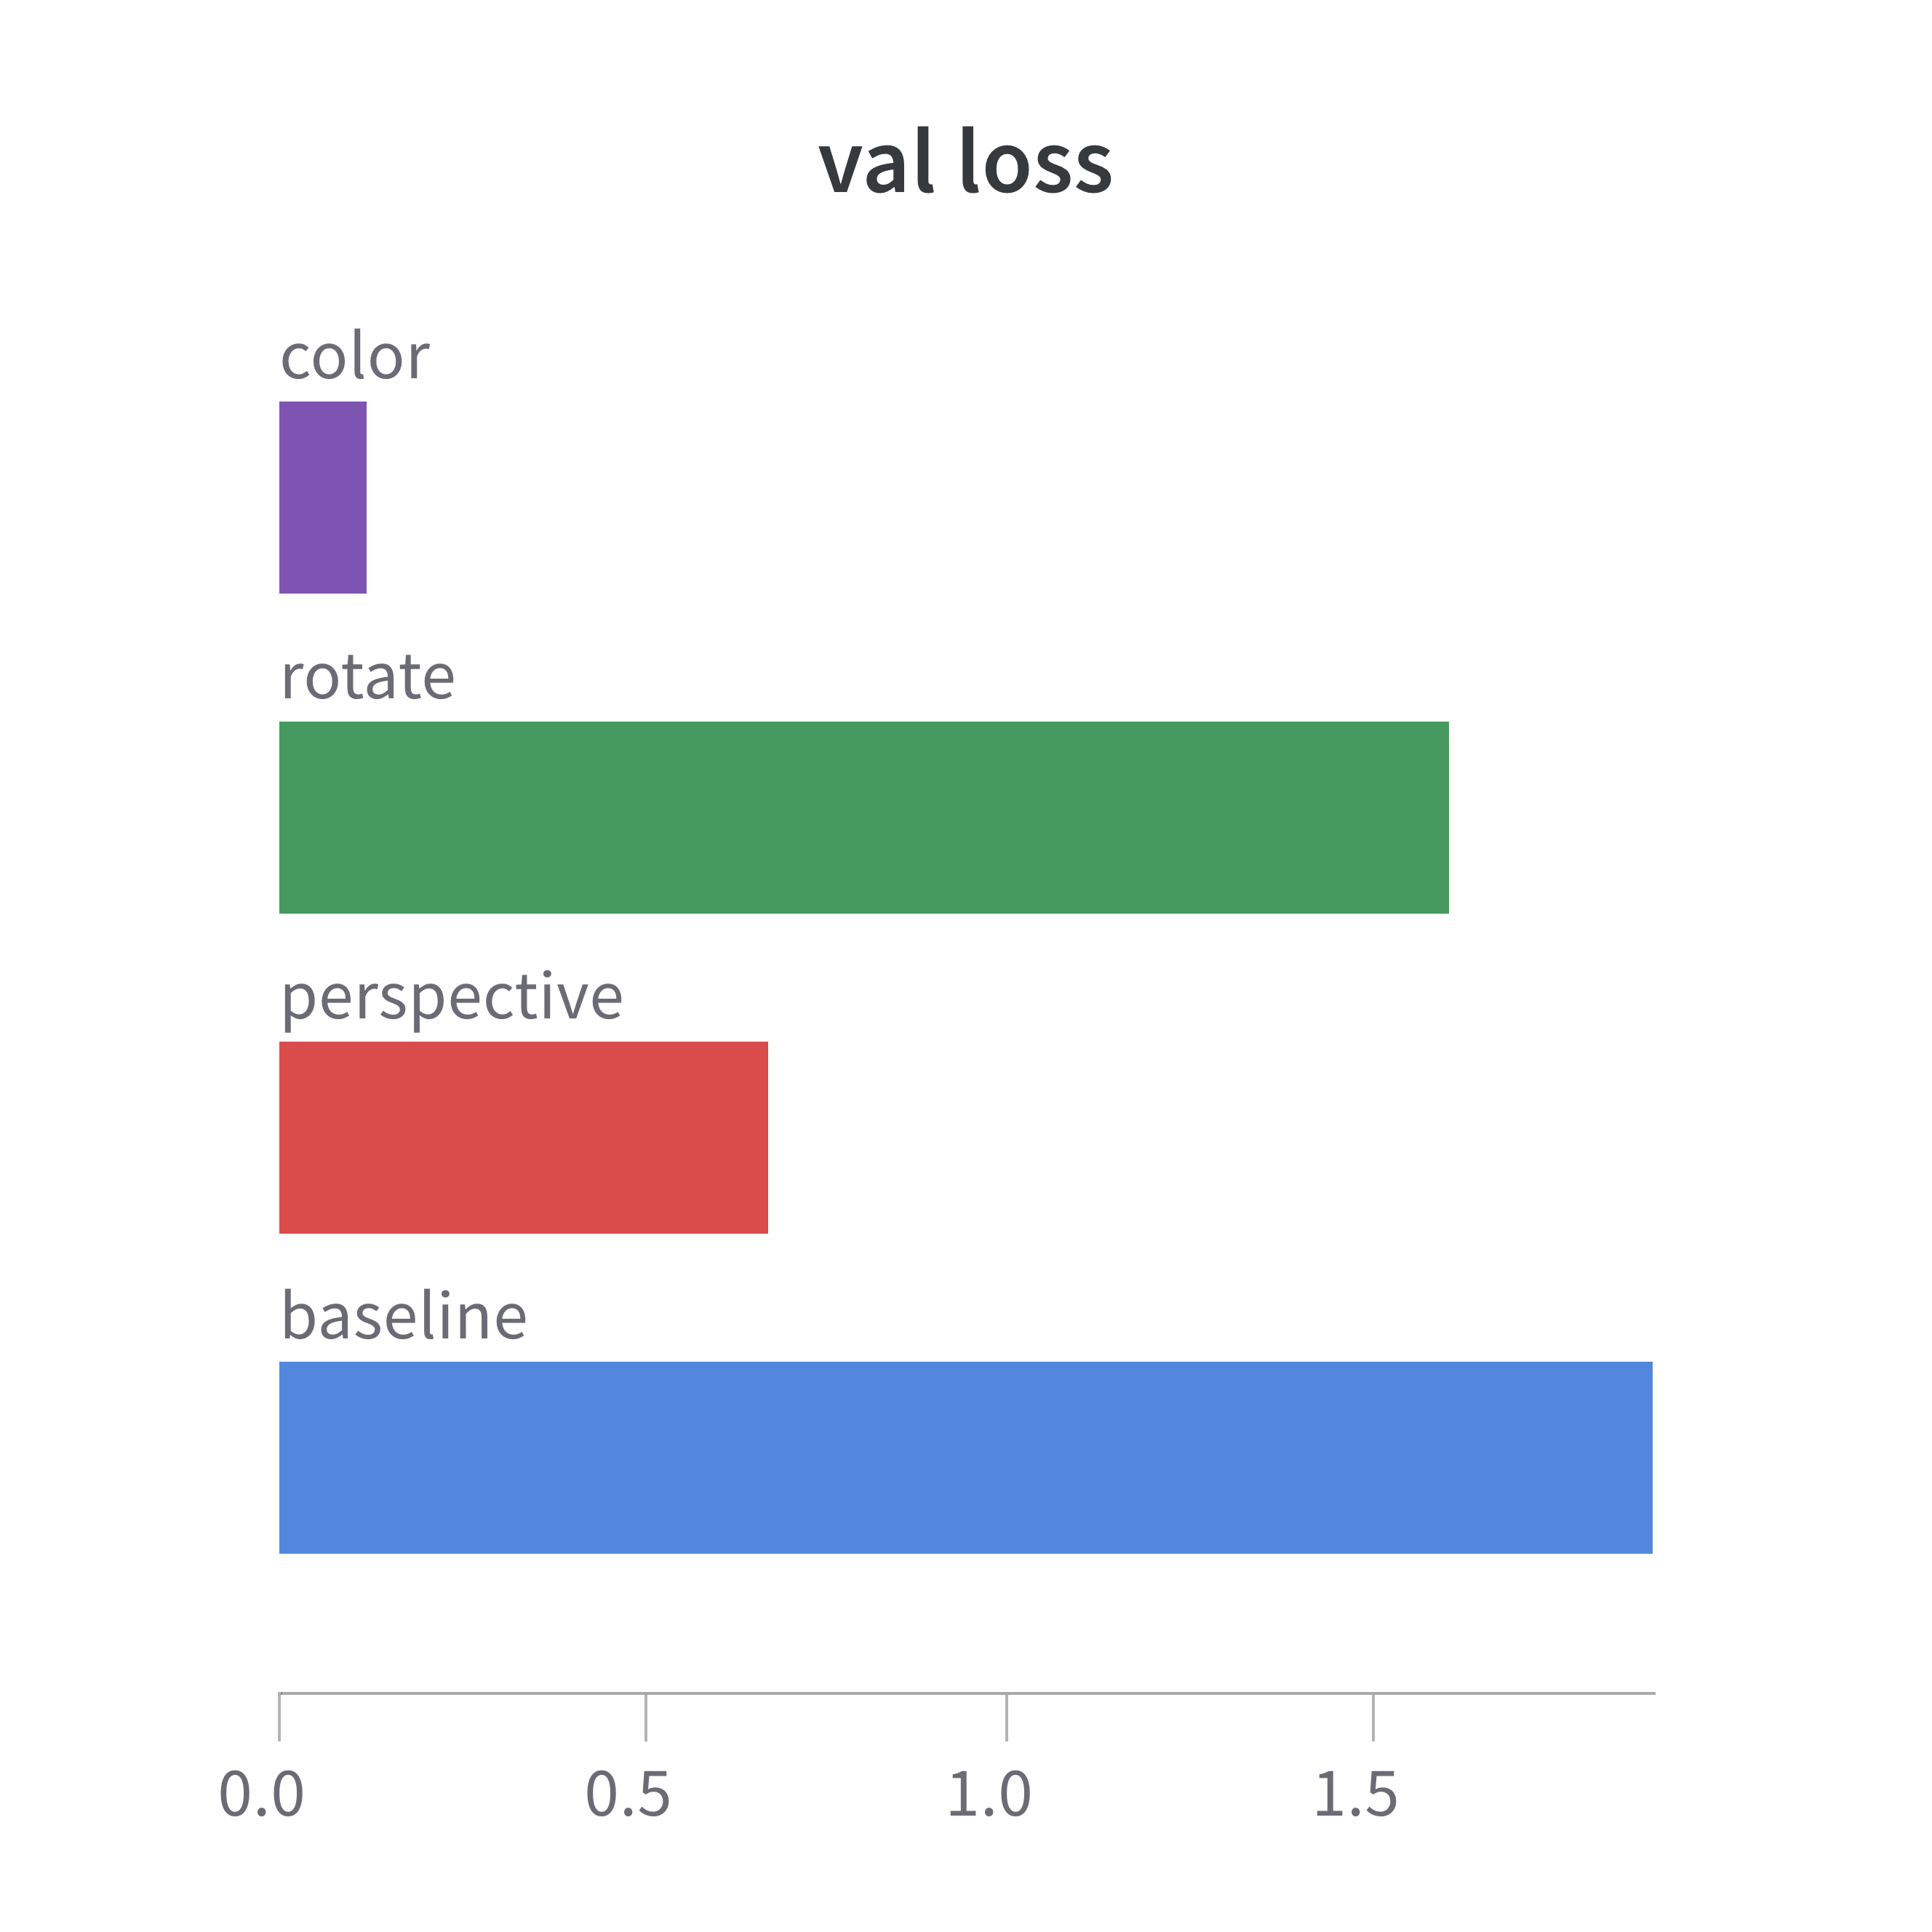
\includegraphics[width=0.75\linewidth]{./img/val_loss.png}
		\caption*{г) график значения функции потерь на валидационной выборке..}
	\end{minipage}
	\caption{Графики значений метрик точности и функции потерь.}
	\label{fig:logsbatch}
\end{figure}

Можно заметить, что значение метрики «точность» у \verb|baseline| модели низкая, по сравнению с другими, это может быть связано с тем, что данная нейронная сеть переобучилась на цвет графиков вероятностных распределений. Значения функции потерь на тренировочной и валидационной выборках крайне большие, что также говорит о низкой обобщающей способности данной модели.

Значение метрики «точность» у \verb|perspective| модели примерно одинаковая на тренировочном и валидационном наборе данных, таким же образом обстоят дела и с метрикой значения функции потерь -- она одна и та же что для тренировочной, что для тестовой выборки. Таким образом, можно сделать вывод, что перспективное преобразование является стабильным и средним по показателям в точности предсказаний.

Рассмотрев \verb|rotate| модель, можно увидеть, что метрика «точность» на тренировочной и валидационной выборках не меняется, в то время как значение функции ошибки на валидационном наборе данных выше, это свидетельствует о том, что хорошие показатели точность могут быть случайны.

Наилучшим образом показала себя \verb|color| модель, которая обучалась на изображениях с изменёнными свойствами. Это видно исходя из уменьшения значения функционала ошибки, а также стабильно высокой точности. 

Таким образом, наилучшим вариантом для дальнейшего использования является \verb|color| модель, которая обучалась на изображениях, подвергшихся изменению контрастности, яркости и насыщенности. 

%%%%%%%%%%%%%%%%%%%%%%%%%% особенности использования нейронной сети %%%%%%%%%%%%%%%%%%%%%%%%%%%
\subsection{Особенности использования нейронной сети для классификации пользовательских изображений}

Для проверки и использования модели в целях классификации пользователем изображений графиков вероятностных функций, необходимо:
\begin{enumerate}
    \item Загрузить \verb|Google Colab Notebook|, файл \verb|color_model.h5| на Google диск в директорию \verb|/content/drive/MyDrive|;
    \item Открыть \verb|Google Colab Notebook|, переключиться на среду выполнения -- GPU;
    \item Выполнить код в ячейка раздела «Необходимое для модели»;
    \item Для классификации изображений перенести их на Google диск, а путь к папке с изображениями записать в переменную \verb|test|;
    \item Выполнить код в ячейке с вызовом функции \verb|give_answers(path)|.
\end{enumerate}
 
%%%%%%%%%%%%%%%%%%%%%%%%%%%%%%%%% ТЕСТИРОВАНИЕ %%%%%%%%%%%%%%%%%%%%%%%%%%%%%%%%%
\section{Тестирование}

Для тестирования решено было взять изображения графиков вероятностных функций двух типов: сгенерированные при помощи библиотеки \verb|SciPy| и отрисованные при помощи библиотеки \verb|Matplotlib|, как это было сделано при сборке данных для обучения и тренировки, однако в данном случае взять другой цвет графика, и изображения графиков вероятностных распределений, которые были нарисованы человеком.

\subsection{Тестирование на сгенерированных изображениях}

На рисунке \ref{fig:gen1} представлены сгенерированные изображения графиков вероятностных функций в дискретном случае, на \ref{fig:gen2} -- непрерывном случае.

Результаты тестирования представлены на рисунке \ref{fig:gen_res}.

\begin{figure}[H]
	\centering
	\begin{minipage}[t]{.4\textwidth}
		\centering
		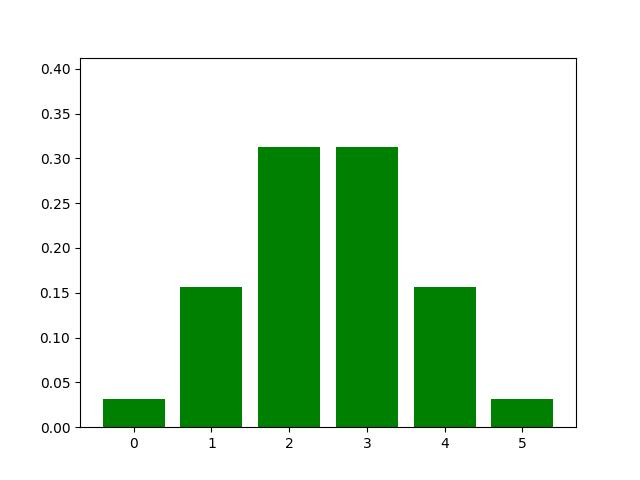
\includegraphics[width=0.75\linewidth]{./img/binom_3.jpg}
		\caption*{а) биномиальное распределение.}
	\end{minipage}
	\noindent
	\begin{minipage}[t]{.4\textwidth}
		\centering
		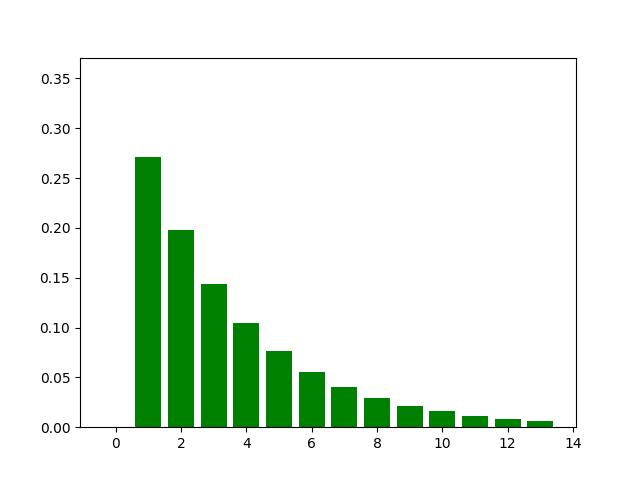
\includegraphics[width=0.75\linewidth]{./img/geom_3.jpg}
		\caption*{б) геометрическое распределение.}
	\end{minipage}
	\begin{minipage}[t]{.4\textwidth}
		\centering
		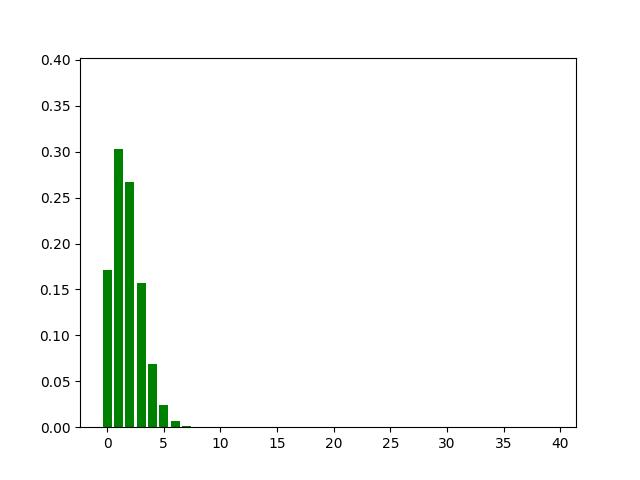
\includegraphics[width=0.75\linewidth]{./img/poisson_3.jpg}
		\caption*{в) распределение Пуассона.}
	\end{minipage}
	\caption{Сгенерированные графики дискретных вероятностных распределений.}
	\label{fig:gen1}
\end{figure}

\begin{figure}[H]
	\centering
	\begin{minipage}[t]{.4\textwidth}
		\centering
		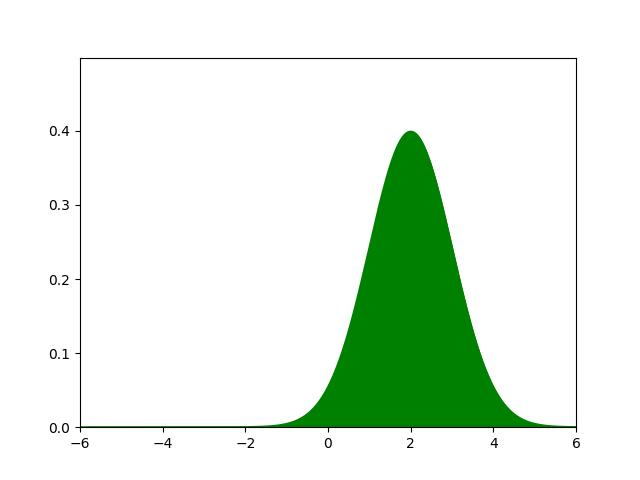
\includegraphics[width=0.75\linewidth]{./img/norm_3.jpg}
		\caption*{а) нормальное распределение.}
	\end{minipage}
	\noindent
	\begin{minipage}[t]{.4\textwidth}
		\centering
		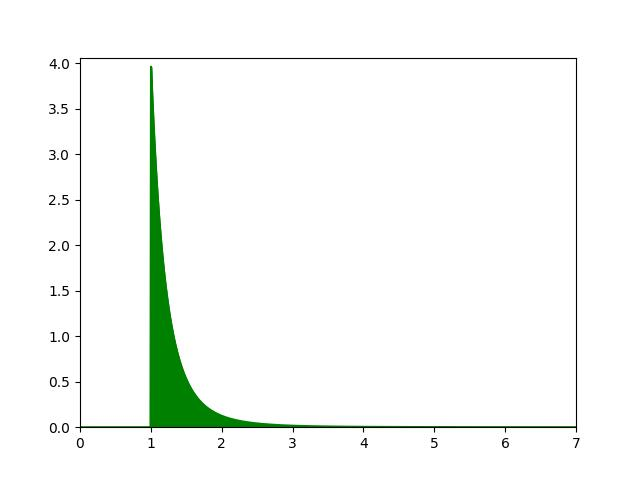
\includegraphics[width=0.75\linewidth]{./img/pareto_3.jpg}
		\caption*{б) распределение Парето.}
	\end{minipage}
	\begin{minipage}[t]{.4\textwidth}
		\centering
		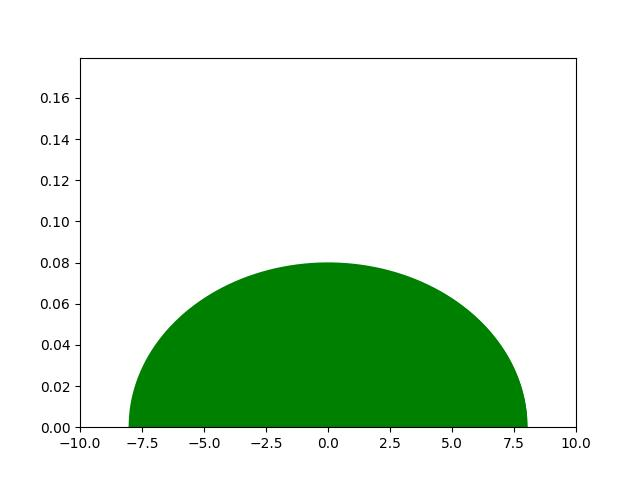
\includegraphics[width=0.75\linewidth]{./img/vigner_3.jpg}
		\caption*{в) полукруговое распределение Вигнера.}
	\end{minipage}
	\caption{Сгенерированные графики непрерывных вероятностных распределений.}
	\label{fig:gen2}
\end{figure}

\begin{figure}[H]
	\centering
	\begin{minipage}[t]{.5\textwidth}
		\centering
		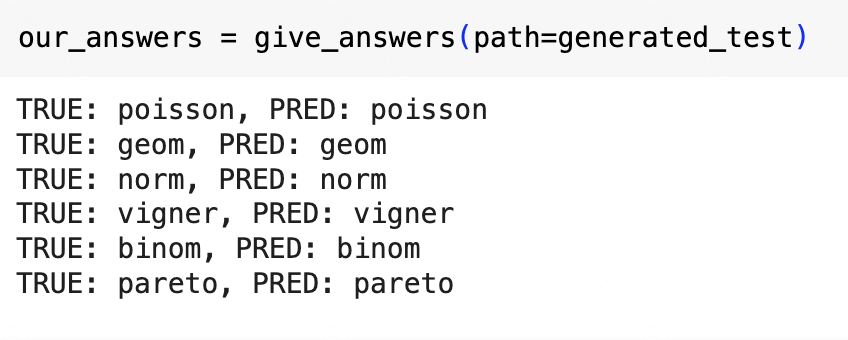
\includegraphics[width=\linewidth]{./img/gen_res.png}
	\end{minipage}
	\caption{Результат тестирования на сгенерированных изображениях.}
	\label{fig:gen_res}
\end{figure}

\subsection{Тестирование на изображениях, нарисованных от руки}
На рисунке \ref{fig:hand1} представлены нарисованные от руки изображения графиков вероятностных функций в дискретном случае, на \ref{fig:hand2} -- непрерывном случае.

Результаты тестирования представлены на рисунке \ref{fig:hand_res}.

\begin{figure}[H]
	\centering
	\begin{minipage}[t]{.35\textwidth}
		\centering
		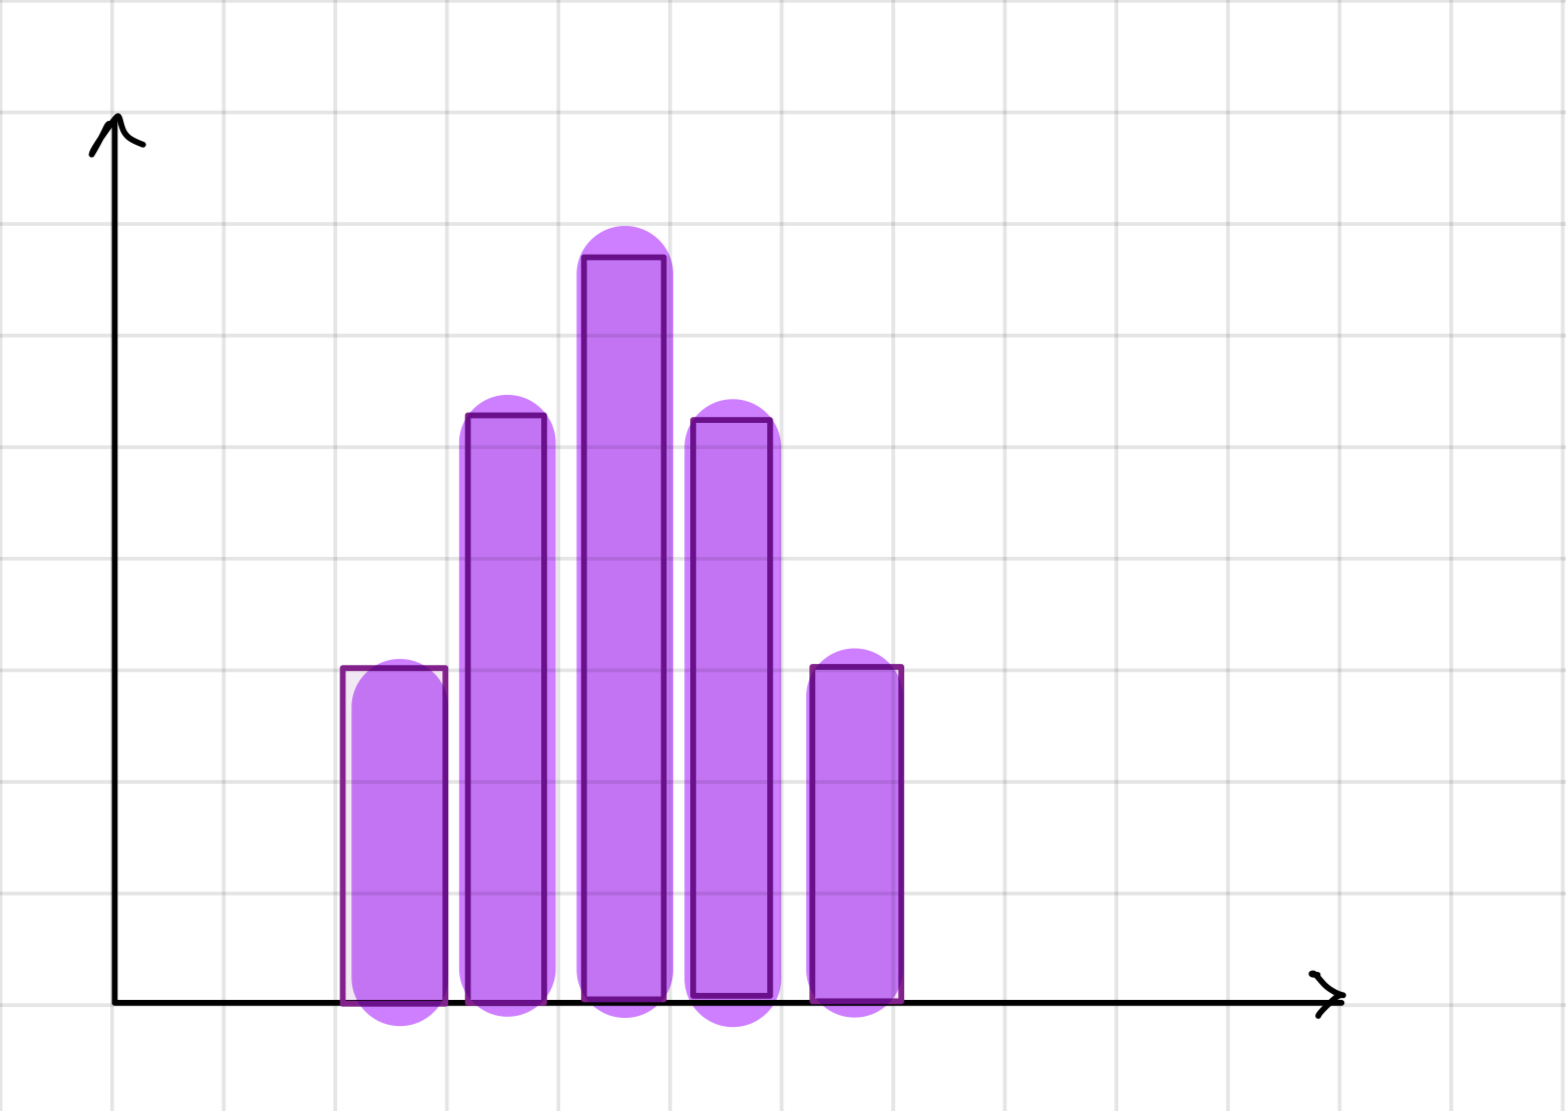
\includegraphics[width=0.7\linewidth]{./img/binom_2.jpg}
		\caption*{а) биномиальное распределение.}
	\end{minipage}
	\noindent
	\begin{minipage}[t]{.35\textwidth}
		\centering
		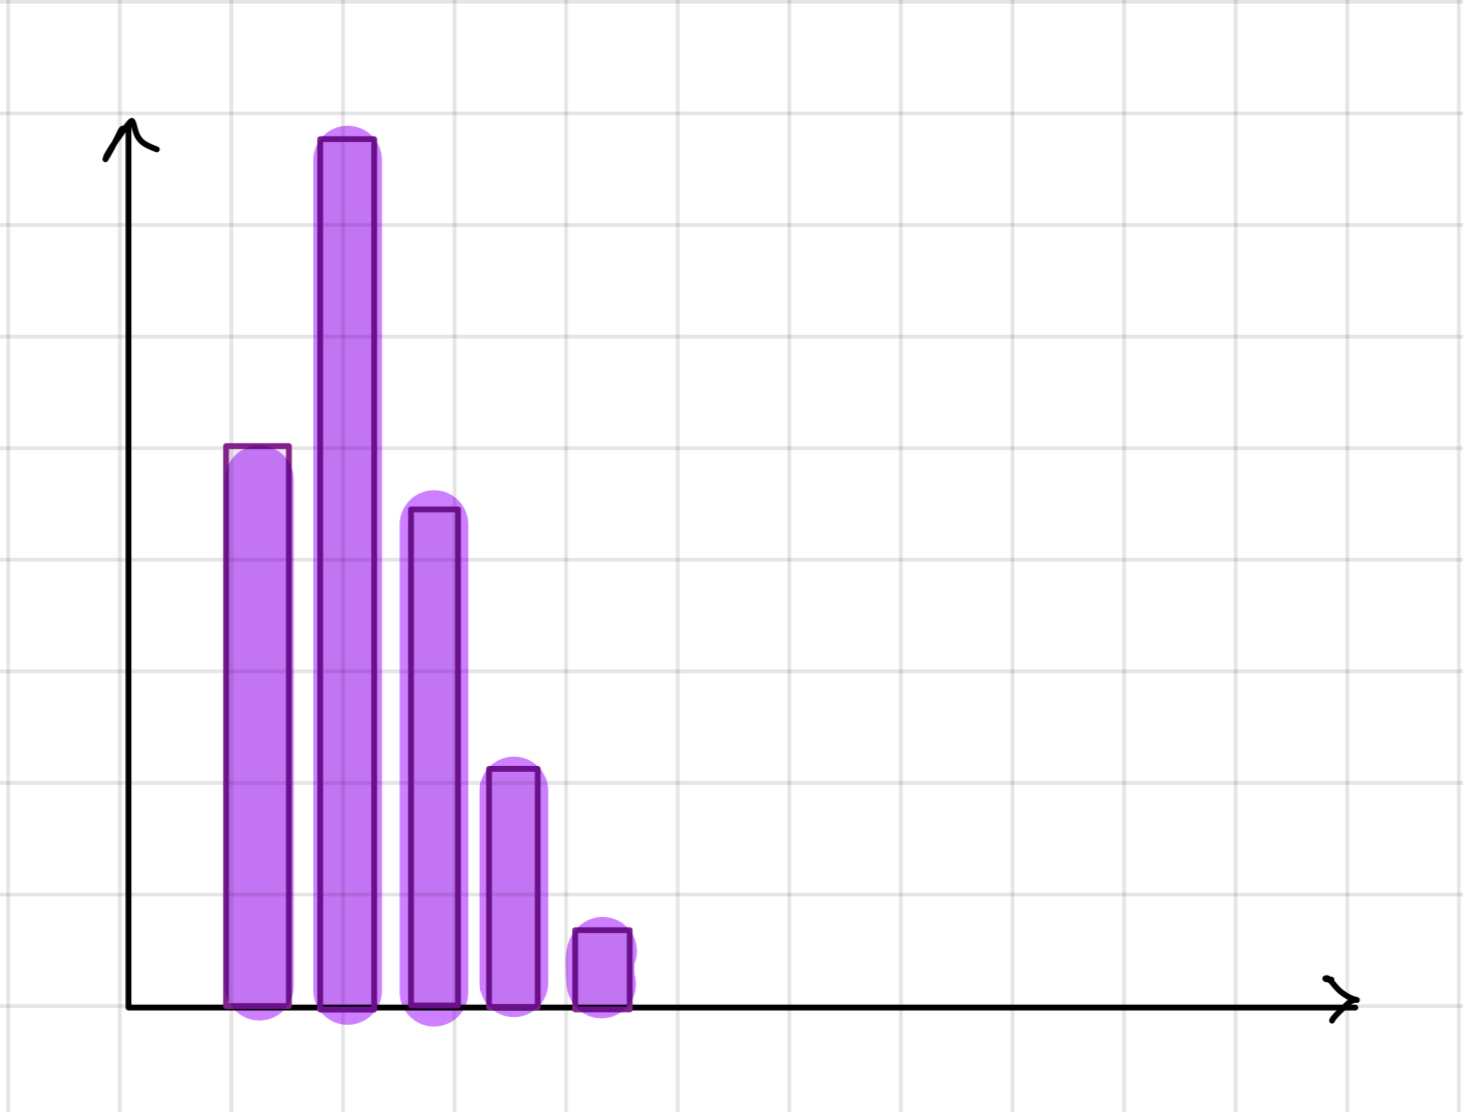
\includegraphics[width=0.7\linewidth]{./img/geom_2.jpg}
		\caption*{б) геометрическое распределение.}
	\end{minipage}
	\begin{minipage}[t]{.35\textwidth}
		\centering
		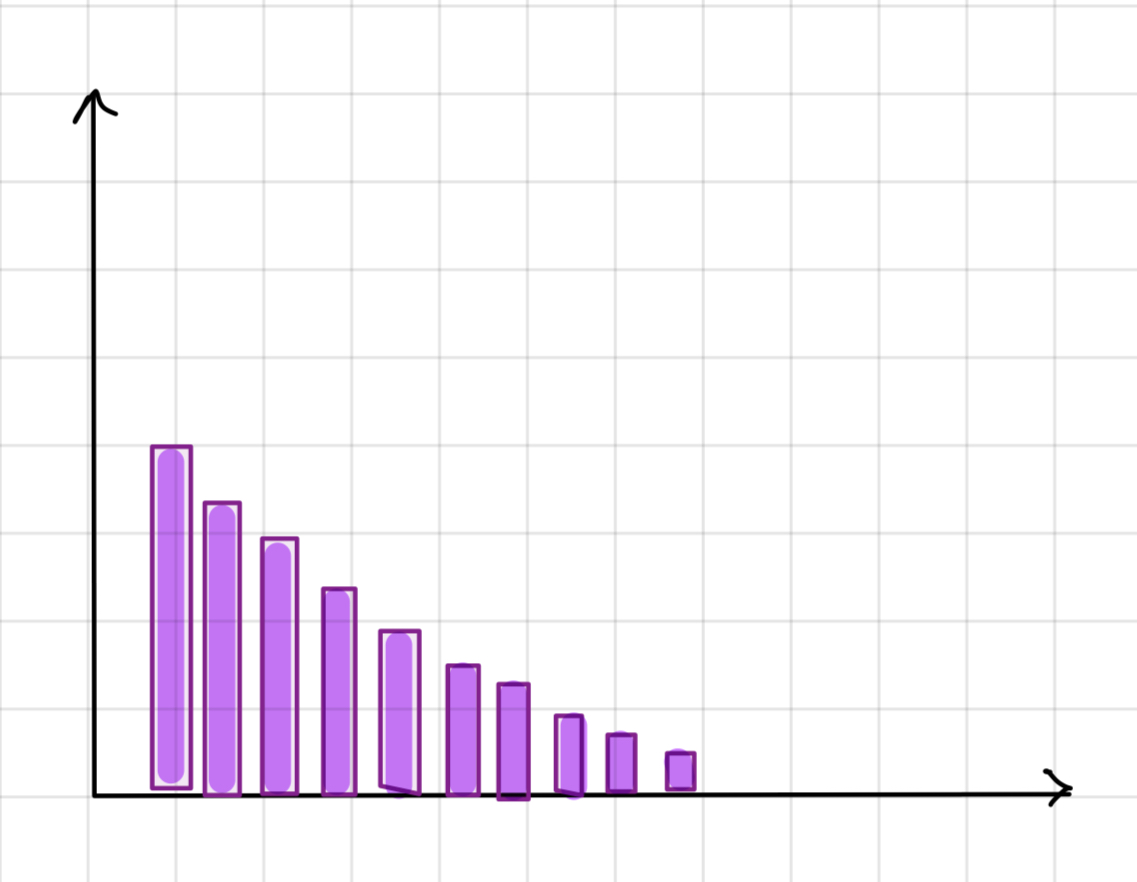
\includegraphics[width=0.7\linewidth]{./img/poisson_2.jpg}
		\caption*{в) распределение Пуассона.}
	\end{minipage}
	\caption{Нарисованные от руки графики дискретных вероятностных распределений.}
	\label{fig:hand1}
\end{figure}

\begin{figure}[H]
	\centering
	\begin{minipage}[t]{.35\textwidth}
		\centering
		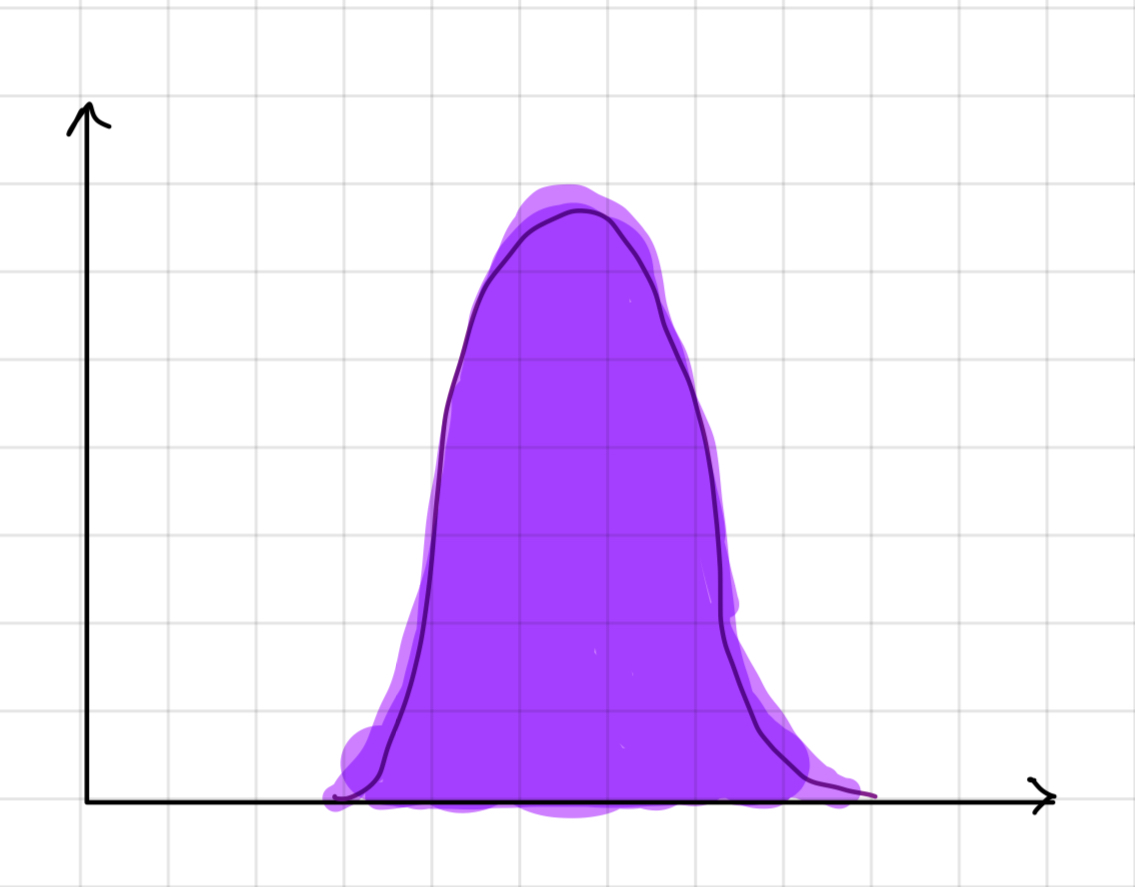
\includegraphics[width=0.7\linewidth]{./img/norm_2.jpg}
		\caption*{а) нормальное распределение.}
	\end{minipage}
	\noindent
	\begin{minipage}[t]{.35\textwidth}
		\centering
		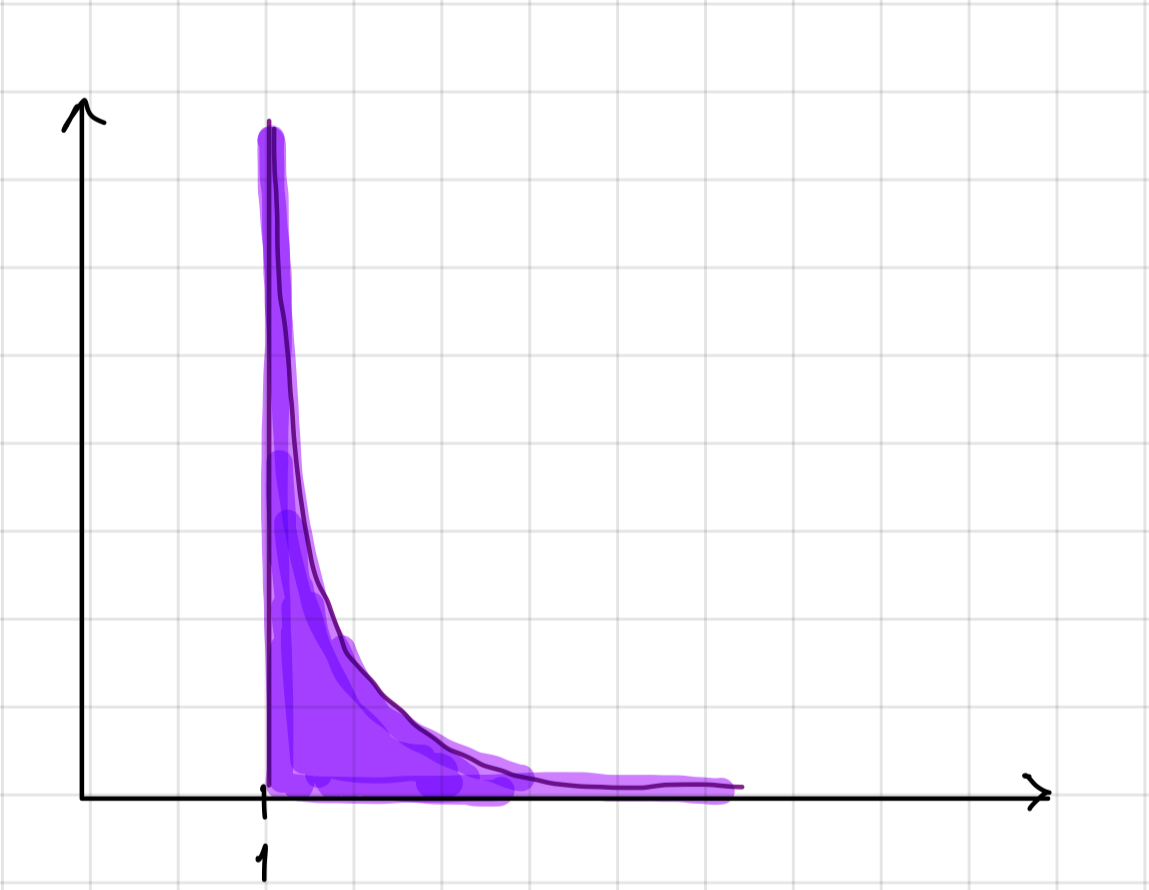
\includegraphics[width=0.7\linewidth]{./img/pareto_2.jpg}
		\caption*{б) распределение Парето.}
	\end{minipage}
	\begin{minipage}[t]{.35\textwidth}
		\centering
		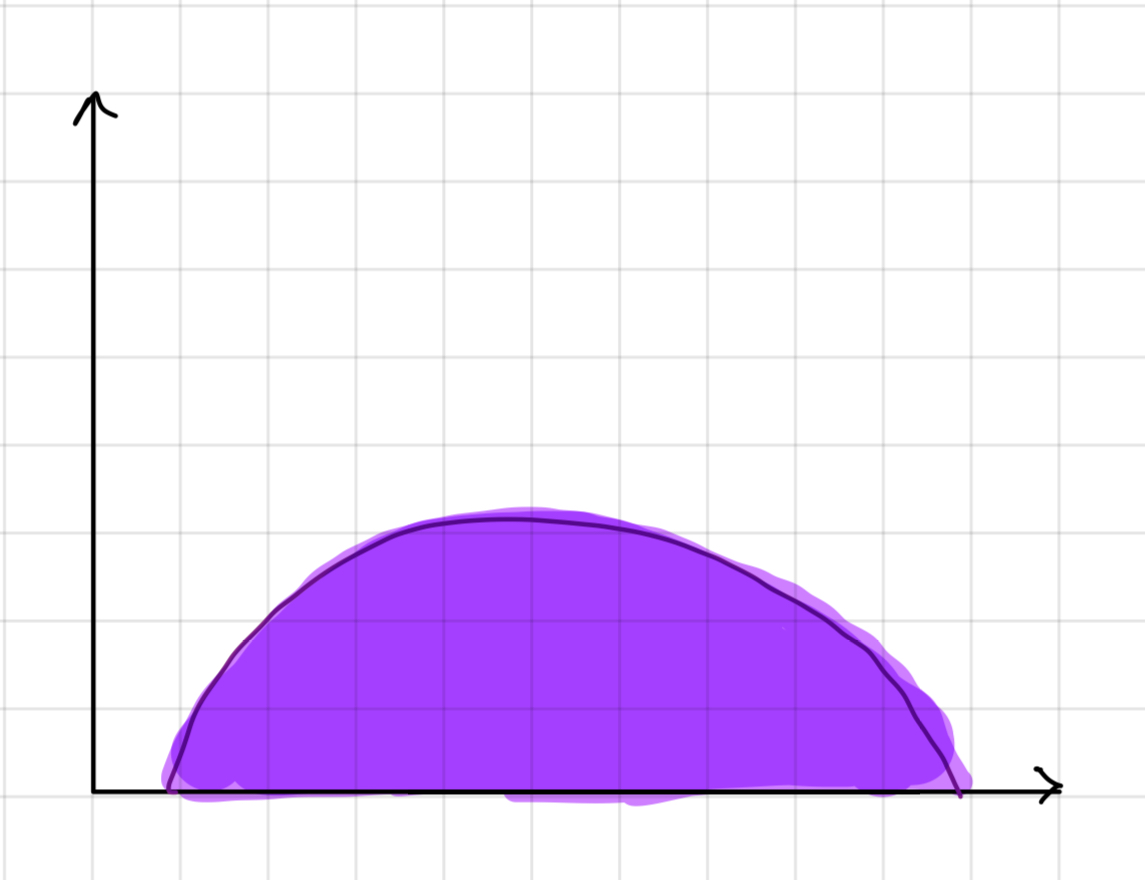
\includegraphics[width=0.7\linewidth]{./img/vigner_2.jpg}
		\caption*{в) полукруговое распределение Вигнера.}
	\end{minipage}
	\caption{Нарисованные от руки графики непрерывных вероятностных распределений.}
	\label{fig:hand2}
\end{figure}

\begin{figure}[H]
	\centering
	\begin{minipage}[t]{.5\textwidth}
		\centering
		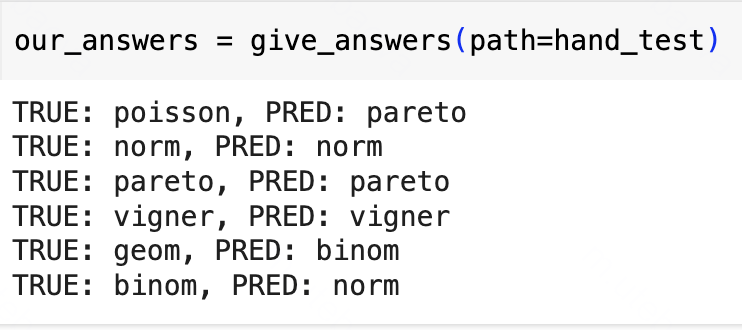
\includegraphics[width=\linewidth]{./img/hand_res.png}
	\end{minipage}
	\caption{Результат тестирования на нарисованных от руки изображениях.}
	\label{fig:hand_res}
\end{figure}

\subsection{Результаты тестирования}
В результате тестирования свёрточной нейронной сети на изображениях, сгенерированных при помощи библиотеки \verb|SciPy| и отрисованных при помощи библиотеки \verb|Matplotlib| получилось так, что классы всех вероятностных распределений предсказаны верно.

При тестировании свёрточной нейронной сети на изображениях графиков вероятностных распределений, которые были нарисованы человеком от руки, модель показала себя хуже, правильно классифицировав лишь три изображения из шести, однако в тех изображениях, в которых нейронная сеть ошиблась, есть крайне похожие графики, например: график биномиального распределения, который крайне похож на график нормального распределения. 

Таким образом, результаты тестирования позволяют сделать вывод о правильности работы разработанной модели, её точности и примерах, на которых нейронная сеть классифицирует изображения неправильно.

%%%%%%%%%%%%%%%%%%%%%%%%%%%%%%%%% ЗАКЛЮЧЕНИЕ %%%%%%%%%%%%%%%%%%%%%%%%%%%%%%%%%
\newpage
\anonsection{ЗАКЛЮЧЕНИЕ}
В ходе выполнения курсовой работы было проведено изучения базовых понятий математической статистики, связанных с вероятностными распределениями, была изучена структура представления изображения в векторном виде, рассмотрены различные операции преобразования над изображениями, произведён анализ существующих методов компьютерного зрения. Рассмотрены различные архитектуры нейронных сетей и методы их оптимизации и обучения.

Основной целью данной курсовой работы была разработка модели машинного обучения для распознавания графиков вероятностных распределений и исследование различных преобразований изображений, направленных на повышение точности прогноза. Результаты выполнения задачи демонстрируют удовлетворительное качество работы модели, что подтверждается проверкой предсказаний нейронной сетью классов графиков вероятностных распределений порождённых программно и человеком, от руки. Разработанное программное решение представляет собой инструмент для анализа и классификации графиков вероятностных распределений.

В заключение, несмотря на достигнутые положительные результаты, существует потенциал для дальнейшего улучшения программы. Это включает в себя расширение набора тренировочных данных, дополнение его графиками, нарисованными от руки, улучшение архитектуры нейронной сети, дообучения её на сложных примерах, более аккуратный подбор параметров обучения. 

\renewcommand\refname{СПИСОК ИСПОЛЬЗОВАННЫХ ИСТОЧНИКОВ}
% Список литературы
\clearpage
%\bibliographystyle{ugost2008s}  %utf8gost71u.bst} %utf8gost705u} %gost2008s}
{\catcode`"\active\def"{\relax}
\addcontentsline{toc}{section}{\protect\numberline{}\refname}%
% \bibliography{biblio} %здесь ничего не меняем, кроме, возможно, имени bib-файла
\printbibliography
}
\newpage
\settocdepth{section}
\anonsection{ПРИЛОЖЕНИЕ А}
\vspace{-30pt}

\begin{listing}[H]
    \caption{Реализация функции визуализации и сохранения графика}
    \label{lst:saveplot}
    \inputminted[style=bw, breaklines, frame=single, fontsize=\footnotesize, linenos=false, xleftmargin=1.5em]{python}{./listings/saveplot.py}
\end{listing}

\begin{listing}[H]
    \caption{Реализация функции распределения изображений по папкам}
    \label{lst:shuffle}
    \inputminted[style=bw, breaklines, frame=single, fontsize=\footnotesize, linenos=false, xleftmargin=1.5em]{python}{./listings/shuffle.py}
\end{listing}

\begin{listing}[H]
    \caption{Реализация функции визуализации изображения}
    \label{lst:show}
    \inputminted[style=bw, breaklines, frame=single, fontsize=\footnotesize, linenos=false, xleftmargin=1.5em]{python}{./listings/show.py}
\end{listing}

\begin{listing}[H]
    \caption{Реализация класса dataset\_statistic}
    \label{lst:dataloader}
    \inputminted[style=bw, breaklines, frame=single, fontsize=\footnotesize, linenos=false, xleftmargin=1.5em]{python}{./listings/dataloader.py}
\end{listing}

\begin{listing}[H]
    \caption{Реализация класса MOLI\_Net}
    \label{lst:molinet}
    \inputminted[style=bw, breaklines, frame=single, fontsize=\footnotesize, linenos=false, xleftmargin=1.5em]{python}{./listings/molinet.py}
\end{listing}

\begin{listing}[H]
    \caption{Реализация класса MOLI\_Net (продолжение)}
    \label{lst:molinet2}
    \inputminted[style=bw, breaklines, frame=single, fontsize=\footnotesize, linenos=false, xleftmargin=1.5em]{python}{./listings/molinet2.py}
\end{listing}

\begin{listing}[H]
    \caption{Реализация функции для обучения на одной эпохе}
    \label{lst:trainepoch}
    \inputminted[style=bw, breaklines, frame=single, fontsize=\footnotesize, linenos=false, xleftmargin=1.5em]{python}{./listings/trainepoch.py}
\end{listing}

\begin{listing}[H]
    \caption{Реализация функции для валидации}
    \label{lst:valepoch}
    \inputminted[style=bw, breaklines, frame=single, fontsize=\footnotesize, linenos=false, xleftmargin=1.5em]{python}{./listings/valepoch.py}
\end{listing}

\begin{listing}[H]
    \caption{Реализация функции для полного цикла обучения}
    \label{lst:full}
    \inputminted[style=bw, breaklines, frame=single, fontsize=\footnotesize, linenos=false, xleftmargin=1.5em]{python}{./listings/full.py}
\end{listing}

\begin{listing}[H]
    \caption{Задание аугментаций и создание выборки}
    \label{lst:test}
    \inputminted[style=bw, breaklines, frame=single, fontsize=\footnotesize, linenos=false, xleftmargin=1.5em]{python}{./listings/test.py}
\end{listing}

\end{document}